\documentclass[11pt]{amsart}

\usepackage{macros, setspace}

\spacing{1.1}

\usepackage{parskip}
\setlength{\parindent}{18pt}
\setlength{\parindent}{0cm}


\author{Owen Gwilliam and Brian R. Williams}
\date{\today}
\title{Holomorphic field theories and higher algebra}

\def\g{{\mathfrak g}}
\def\U{{\rm U}}
\def\mc{\mathcal}
\def\mcol{\, | \,}
\def\ot{\otimes}
\def\Disj{\operatorname{Disj}}
\def\Open{\operatorname{Open}}
\def\Vect{\operatorname{Vect}}
\def\jou{{\mathtt{j}}}
\def\bgamma{{\mathbf{\gamma}}}
\def\bbeta{{\mathbf{\beta}}}
\def\CDO{{\cC\cD}}
\def\SU{{\rm SU}}
\def\sfa{\mathsf{a}}
\def\del{\partial}
\def\til{\Tilde}
\def\Sol{\text{Sol}}
\def\Spec{\text{Spec}}

\renewcommand{\op}{\operatorname}
\def\lie#1{\ensuremath{\mathfrak{#1}}}

\def\brian#1{{\textcolor{blue!65!red}{BW: {#1}}}}
\def\owen#1{{\textcolor{violet!65!black}{OG: {#1}}}}

%\usepackage[upint]{stix}

\begin{document}

\dedicatory{To Yuri Manin, with gratitude and admiration.}

\maketitle
\tableofcontents

\owen{mention some history (e.g., Manin! Donaldson-Thomas, Nekrasov) and some recent work (CPTVV, Pridham, etc) but then explain our focus: higher analogs of VOAs and finding mathematical analogs of physics}

\owen{Notation to explain: dg = differential graded, PDE = partial differential equations}

\brian{we need to make sure to cite nekrasov}


\section{What is a holomorphic field theory? Why study them?}

The most important field theories in physics involve a metric on a manifold (whether Riemannian or Lorentzian), and hence geometry has long had a clear role in physics.
In recent decades attention has expanded to include {\em topological} field theories (or TFTs), 
in which --- to simplify --- only the underlying smooth topology of the manifold matters.
There are, however, theories that depend on a complex structure on the manifold,
and as one might hope, these are particularly beautiful, 
just as complex variables is a particularly beautiful wing of analysis.
In essence, such {\em holomorphic} field theories have variational partial differential equations (i.e., ``equations of motion'') that are holomorphic:
the PDE only involves derivatives in the holomorphic coordinates (i.e., the $\partial/\partial z_j$) and has holomorphic coefficients.
These theories admit independent motivations from mathematics and physics,
which we sketch before giving more careful definitions.

The mathematical motivation is simple:
for most classical holomorphic field theories, the solutions to the equations of motion form a moduli space of natural interest to complex geometers,
and it is natural to hope that its quantization is equally interesting.
A well-known example is holomorphic Chern-Simons theory,
which lives on a Calabi-Yau 3-fold~$X$ and involves the {\em derived} moduli space $\RR\Bun_G(X)$ of holomorphic principal $G$-bundles on~$X$.
As a somewhat mundane example, let $\RR\Hol(X,Y)$ denote the derived moduli space of holomorphic maps from some complex manifold $X$ to another complex manifold $Y$.
(For $Y = V$ a vector space, a ``derived'' enhancement is familiar as the higher dimensional cohomology $H^*(X, \cO) \otimes V$.)
One can take a ``shifted cotangent bundle'' $T^*[-1] \RR\Hol(X,V)$,
and this derived moduli space encodes solutions to
a theory known as the $\beta\gamma$ system with target $V$.
(The name is silly: it's due to the original notation people used.)
Every question one asks about the classical physics of the $\beta\gamma$ theory translates into a question about this moduli space.
Other classes of examples are afforded by holomorphic variants of familiar AKSZ $\sigma$-models; the relevant moduli space being the derived mapping space between complex manifolds. 

A physical motivation comes from supersymmetric field theories, 
which (loosely speaking) are theories on $\RR^n$ whose symmetries include not only the isometries of $\RR^n$, but an extension to a Lie supergroup known as a super Poincar\'e group.
%The relevant extension is often labeled by $\cN=1, 2,$ and so on, 
%with larger $\cN$ denoting a bigger supergroup. 
Thanks to the enhanced symmetry, such theories can often be understood in greater detail than non-supersymmetric theories.
The relevance to the models we study is that supersymmetric theories admit ``twists'' (in essence, deformations) that are holomorphic field theories, 
even when they do not admit twists to TFTs (such as the famed A- and B-models of mirror symmetry) \cite{CosHol}.
As an example, four-dimensional minimally supersymmetric Yang-Mills theory admits no topological twist, but does admit a twist to holomorphic field theory whose moduli space is described, in part, by the moduli space of holomorphic $G$-bundles~$\RR \Bun_G(X)$. 
It is natural to wonder how the myriad tools and computations deployed on the supersymmetric theory carry over to this twist and conversely whether information can flow back from a holomorphically twisted theory to the untwisted one, 
much as TFTs have enriched the understanding of supersymmetric theories.
In short, a holomorphic twist contains the ``holomorphic sector'' of the untwisted theory just as a topological twist contains its ``topological sector.''

As a final motivational remark, we note in one complex dimension (i.e., working on Riemann surfaces), holomorphic field theories appear as chiral conformal field theories (CFTs) on two-dimensional manifolds --- whose manifestations in mathematics include vertex algebras, affine Lie algebras, and loop groups --- and have had a strong impact in mathematics.
It is natural to explore higher-dimensional analogs.

The overarching goal of this paper is \owen{continue}
a cluster of projects is to bring into sharp mathematical form some of the deep insights into gauge theory offered by physics.
So far, most mathematical effort has focused on classical gauge theory,
but the quantum aspects are profoundly interesting.
We expect that these holomorphic examples will be particularly tractable and beautiful but also useful in offering insights even for non-holomorphic theories.

\subsection{Preliminary notions}


\brian{complex geometry, dolbeault, dg stuff.}

A theory is usually described, in part, in terms of a space of fields which comprise some possibly nonlinear space like a mapping space or the space of connections. 
In perturbative field theory, which describes the formal neighborhood of the theory at points in such spaces, the fields $\Phi$ are typically described by the smooth sections of a bundle on spacetime.
The equations of motion which dictate the dynamics of the particular model are encoded by a partial differential equation heuristically of the form 
\[
\sum_{k \geq 1} D_k(\Phi,\ldots,\Phi) = 0 ,
\]
where $D_k$ is a $k$-ary polydifferential operator.
As an example of a Euclidean theory, the $\phi^4$-theory on a Riemannian four-manifold $M$ is described by the equation
\[
\Delta \phi + \frac{1}{3!} \phi^3 = 0 
\]
where $\Phi = \phi$ is simply a smooth function on $M$.
 
In a {\em holomorphic theory} one starts with a complex manifold $X$ as the spacetime.
This means, in part, that the complexified tangent bundle of $X$ decomposes as a sum of vector bundles $\T_X \oplus \Bar{\T}_X$ where $\T_X$ (respectively $\Bar{T}_X$) is the holomorphic (respectively anti-holomorphic) tangent bundle.
In local coordinates sections of $\T_X$ have the form $f^i \del / \del z_i$ whereas sections of $\Bar{\T}_X$ have the form $f^i \del / \del \zbar_i$. 

Globally, holomorphic theories are described like in the usual case by mapping spaces or spaces of connections.
The key feature in a holomorphic theory is that the equations of motion dictate that fields be holomorphic.
Perturbatively, where fields are sections of some holomorphic vector bundle $V$, we can make this precise. 
Prescribing a holomorphic structure on a vector bundle $V$ is equivalent to the data of a $\dbar$-operator
\beqn
\dbar \colon \Omega^{0,q}(X, V) \to \Omega^{0,q+1}(X,V) 
\eeqn
where $\Omega^{0,q}(X,V)$ is the space of smooth sections of the vector bundle $\wedge^q\Bar{T}_X^* \otimes V$. 
Holomorphicity of $V$ boils down to the requirement that $\dbar \circ \dbar = 0$.
The Dolbeault complex of $V$ is the resulting complex $(\Omega^{0,\bu}(X, V), \dbar)$ where $\Omega^{0,q}(X,V)$ sits in degree $+q$.
A standard result in complex geometry is that the Dolbeault complex is a resolution for the sheaf of holomorphic sections of the holomorphic vector bundle $V$.
In the case that $V$ is the trivial bundle $\ul{\CC}$ the Dolbeault complex $\Omega^{0,\bu}(X)$ is a resolution for the sheaf of holomorphic functions on $X$.

The fields of a holomorphic theory are given by elements of the Dolbeault complex $\Omega^{0,\bu}(X,V)$.
The equations of motion in a holomorphic theory take the form
\beqn
\dbar \Phi + \sum_{k \geq 1} D_k(\Phi,\ldots,\Phi) = 0 ,
\eeqn
where $D_k$ are $k$-ary {\em holomorphic} polydifferential operators.
This means that in local coordinates $D_k$ only depend on the holomorphic coordinates $\{z_i\}$ and involve only holomorphic derivatives $\del / \del z_i$.


\subsection{Precise definitions}

Let us begin with the example of holomorphic Chern--Simons theory, 
which we have already said describes the moduli space of Maurer--Cartan elements describe deformations of the trivial holomorphic $G$-bundle. 
When $X$ is a Calabi--Yau three-fold and $\fg$ is equipped with an invariant pairing $\<\cdot , \cdot \>$, 
this formal moduli space has a very special property: 
it arises from the variational problem of an action functional, namely
\beqn
S = \int_X \Omega \wedge {\rm CS}(A) 
\eeqn
where $\Omega$ is the holomorphic volume form and 
\beqn
{\rm CS}(A) = \frac12 \< A ,\d A \> + \frac16 \<A , [A,A]\>
\eeqn
is the Chern--Simons Lagrangian for the connection $(0,1)$-form $A$.
Notice that due to the presence of the holomorphic volume form $\Omega$ on the $\dbar$ operator contributes to the kinetic term and so the action can be written as 
\beqn
S = \int_X \Omega \wedge \left(\frac12 \< A ,\dbar A \> + \frac16 \<A , [A,A]\>\right) .
\eeqn

We turn to a formal definition underpinning the formal moduli spaces of the holomorphic field theories that we will be considering. 

\begin{dfn}
A {\em holomorphic dg Lie algebra} on a complex manifold $X$ is
\begin{itemize}
\item a graded holomorphic vector bundle $V$ on $X$ whose sheaf of holomorphic functions is $\cV^{hol}$, and
\item a holomorphic differential operator $Q^{hol} \colon \cV^{hol} \to \cV^{hol}$ of cohomological degree one and a holomorphic bidifferential operator $[\cdot,\cdot] \colon \cV^{hol} \times \cV^{hol} \to \cV^{hol}$. 
\end{itemize}
This data is required to endow $(\cV^{hol}, Q^{hol}, [\cdot,\cdot])$ with the structure of a dg Lie algebra.
\end{dfn}

Any holomorphic vector bundle has an associated Dolbeault complex $\Omega^{0,\bu}(X,V)$. 
If $V$ is a holomorphic dg Lie algebra, 
then $\Omega^{0,\bu}(X, V)$ is a dg Lie algebra. 
The differential is of the form $\dbar + Q^{hol}$ and the bracket is given by extending the bracket on $\cV^{hol}$ with the wedge product of differential forms. 

Formal moduli spaces arise from the space of Maurer--Cartan elements of a dg Lie algebra.
In our case, this dg Lie algebra will always be of the form $\Omega^{0,\bu}(X, V)$.
For example, the Maurer--Cartan elements of the dg Lie algebra $\Omega^{0,\bu}(X, \fg)$ recovers formal deformations of the trivial holomorphic $G$-bundle.  
This arises from the holomorphic Lie algebra on $X$ whose underlying vector bundle is trivial with fiber $\fg$. 

As another example, consider the holomorphic tangent bundle $V = \T_X$. 
The Lie bracket of vector fields endows this with the structure of a holomorphic Lie algebra (with zero differential). 
A Maurer--Cartan element in $\Omega^{0,\bu}(X, \T_X)$ is an element $\mu \in \Omega^{0,1}(X, \T_X)$ satisfying the equation
\[
\dbar \mu + \frac12 [\mu,\mu] = 0 .
\]
This recovers the classical picture describing formal deformations of complex structures on~$X$.


%this section aimed at mathematicians
%emphasize connection with (derived) complex geometry

\subsection{Examples}

In traditional physics there are a few basic types of field theories, 
and they can be assembled into combinations in natural ways,
of which the Standard Model offers a nice example.
The basic types are\footnote{For the experts, we remark that we focus above on the core field content, and ignore (just for the moment!) issues like gauge transformations and the associated ghost fields.}
\begin{itemize}
\item {\em Scalar} field theories where the fields are maps from $M$ to a vector space $V$, or natural generalizations like taking sections of a vector bundle $V \to M$. The Higgs boson appears as part of a scalar field theory.
\item {\em Fermionic} field theories where the fields are maps from $M$ to an {\em odd} vector space or, typically, a section of a spinor bundle. Such theories are often used to describe matter, such as electron fields.
\item {\em Gauge} field theories where the fields are connections on a principal $G$-bundle over $M$, with $G$ a Lie group. The Yang--Mills theories for the electroweak and strong forces are examples.
\item $\sigma$-{\em models} where the fields are maps from $M$ into a manifold~$X$. (One can view these as generalizations of scalar field theories.)
\item {\em Gravity} theories where the fields are metrics on $M$, or something that similarly controls the geometry of $M$. Einstein's theory is a paradigmatic example.
\end{itemize}
The Standard Model involves the first three types,
and the different fields interact in intricate ways.

There are holomorphic versions of all these basic types, 
and we now spell out some simple examples.
To give the readers --- possibly a mixed audience of mathematicians and physicists --- some feel for the examples, 
we describe them in several ways: 
in terms of PDE and action functionals but also as moduli spaces.
We do not offer a thorough justification of the dictionary, for which see \owen{cite who?}

For an example that mixes several types and that is a holomorphic analog of quantum chromodynamics (QCD), the theory that governs the strong force and quarks,
see Section~\ref{sec: seiberg}.
One motivation for us to explore holomorphic field theories is that one can translate physical insights and conjectures (such as Seiberg duality) into surprising predictions in the holomorphic setting,
which is typically much cleaner and more accessible.
(One might also hope that progress in the holomorphic setting then feeds back useful insights to physics.)


\subsubsection{Holomorphic scalar field theories}

The most elementary holomorphic field theory is a generalization of the so-called `$\beta\gamma$ system' which is primarily studied in the context of string theory.
The input data is simply a complex manifold $X$ of arbitrary complex dimension $n$ together with a (super) holomorphic vector bundle $V$ on $X$.
The fields of the theory consist of pairs 
\begin{align*}
\gamma & \in \Gamma(X,V)\\
\beta & \in \Omega^{n,n-1}(X,V^*) .
\end{align*}
The action functional is 
\beqn
\int_X \beta \wedge \dbar \gamma 
\eeqn
which utilizes the natural pairing between $V$ and $V^*$. 
The theory is free, just like the ordinary $\beta\gamma$ system on Riemann surfaces.

Notice that there is a linear symmetry present in the above action given by shifting $\beta$ by a $\dbar$-exact form
\beqn
\beta \mapsto \beta + \dbar \eta , \quad \eta \in \Omega^{n,n-2}(X,V^*)
\eeqn
For this model to be well-posed at the quantum level we must include the ghosts $\eta$.
Further, $\eta$ can be shifted by an exact form in a way that does not effect the above gauge transformation, so we must also include ghosts for ghosts, etc..

\subsubsection{Holomorphic gauge theories}

We have already met holomorphic Chern--Simons theory, which is defined on Calabi--Yau three-folds.
There is a related holomorphic gauge theory which is defined in arbitrary complex dimensions and does not require the data of a Calabi--Yau structure. 

If $n$ is the complex dimension of $X$, the fields consist of pairs $(A,B)$ where $A$ is a $(0,1)$ connection on a principal $G$-bundle $P \to X$ and
\beqn
B \in \Omega^{n,n-2}(X, \fg_P^*) ,
\eeqn
where $\fg_P$ is the adjoint bundle of $P$. 
The action functional is 
\beqn
S(A,B) = \int_X B \wedge F_A 
\eeqn
where $F_A$ is the curvature of the connection $A$.
From this formula, it is clear that the model we are describing is a holomorphic analog of topological $BF$ theory. 
Notice that by form types this action can be written as
\beqn
S(A,B) = \int_X B \wedge \left(\dbar A + \frac12 [A,A] \right) .
\eeqn


\subsubsection{Holomorphic $\sigma$-models}

If $X,Y$ are any two complex manifolds there is a theory whose fields consist, in part, of the derived moduli space of smooth maps $\RR {\rm Map}(X,Y)$ and whose equations of motion dictate that such maps be holomorphic.
This is a nonlinear generalization of the $\beta\gamma$ system we just introduced. 
  
The precise space of fields, in cohomological degree zero, consist of pairs $(\gamma, \beta)$ where $\gamma \colon X \to Y$ is a smooth map and 
\[
\beta \in \Omega^{n,n-1}(X, f^* \T^*_Y) 
\]
where $\T^*_Y$ is the holomorphic cotangent bundle of $Y$. 
The action functional is the familiar one
\beqn
\int_X \beta \dbar \gamma .
\eeqn 


\subsubsection{Holomorphic gravity}

Perturbatively, any model of gravity describes, in part, deformations of the moduli space of metric structures on a given manifold. 
There is a holomorphic avatar of this which describes deformations of complex structure.
The fields consist of pairs $(\mu, \eta)$ where
\begin{align*}
\mu & \in \Omega^{0,1}(X, \T_X) \\
\nu & \in \Omega^{0,n-2}(X, K_X \otimes \T^*_X) .
\end{align*}
The action functional is
\beqn
\int_X \left(\eta \dbar \mu + \frac12 \eta [\mu,\mu]\right)
\eeqn
where $[\mu, \mu] \in \Omega^{0,2} (X, \T_X)$ stands for the Lie bracket of holomorphic vector fields extended to the Dolbeault valued sections of $\T_X$ in the natural way.

In complex dimension $3$ there is a related theory, called Kodaira--Spencer theory, which only consists of the field $\mu$ describing the complex structure in the above example.
Let $X$ be a complex threefold equipped with a Calabi--Yau structure where we denote by $\Omega \in \Omega^{3,hol}(X)$ the holomorphic volume form.
Kodaira--Spencer theory is the holomorphic theory whose fields consist of $(0,1)$ forms on $X$ with values in the holomorphic tangent bundle $\T_X$
\beqn
\mu \in \Omega^{0,1}(X,\T_X) .
\eeqn 
A crucial assumption of this model is that we must assume that $\mu$ preserve the holomorphic volume form $\Omega$, meaning its divergence vanishes ${\rm div}_\Omega \mu = 0$.
The action functional is very similar to the Chern--Simons action
\beqn
S(\mu) = \int_X \left(\frac12 \mu \dbar \del^{-1} \mu + \frac13 \mu^3\right) .
\eeqn
The integrand is not defined globally.
In the integral we use the Calabi--Yau form to identify the integrand with 
\brian{finish}

\subsection{Local version and examples from supersymmetric field theories}

%this section aimed at physicists
%twists of SUSY theories
%Owen has some nice thoughts about globalization as it related to SUSY/THF.

There is the following local characterization of a holomorphic field theory which allows us to connect directly to supersymmetric field theories. 
Suppose that our spacetime is $\CC^n = \RR^{2n}$ and assume that the theory we are considering is translation invariant, meaning that there is an action buy the $2n$-dimensional Lie algebra spanned by the vector fields $\del / \del {z_i}, \del / \del {\zbar_i}$ for $i=1,\ldots,n$. 
In a holomorphic theory we require that the anti-holomorphic vector fields $\del / \del {\zbar_i}$ act homotopically trivial. 
In the derived world this is prescribed by the data of homotopy trivializations for such vector fields. 

Any even dimensional supersymmetric field theory produces a holomorphic field theory through a process called twisting,
so we have a wealth of examples to study that are intimately connected to theories of genuine interest in physics.\footnote{Strictly speaking, this requires the existence of of more than two chiral supercharges. So, theories with 2d $\cN = (n,m)$ supersymmetry, $n,m \leq 1$, do not admit holomorphic twists.}
As we will explain later, many interesting phenomena for supersymmetric theories have analogs in holomorphic field theory.
 
By definition, a supersymmetric field theory on $\RR^d$ is a theory that is acted upon by a super Poincar\'{e} algebra. 
We focus on Euclidean field theories and work in Riemannian signature,
hence for us the ``super Poincar\'{e} algebra'' is a super Lie algebra of the form
$\mathfrak{so}(d) \ltimes \ft$
where $\ft$ is the super Lie algebra of {\em supertranslations} whose even part $\ft^0 = \RR^d$ is the Lie algebra of ordinary translations and whose odd part $\ft^1$ is a sum of spin representations. 
While the Lie algebra $\RR^d$ of ordinary translations is abelian, the Lie algebra $\ft$ carries a nontrivial (super) Lie bracket,
and this Lie bracket is defined in terms of a $\mathfrak{so}(d)$-equivariant non-degenerate symmetric pairing
\beqn
\label{e:Gamma}
\Gamma \colon {\rm Sym}^2(\ft^{1}) \to {\rm Sym}(\ft^0) \cong \RR^d 
\eeqn
by the formula $[\cQ, \cQ'] = \Gamma(\cQ, \cQ')$. 

By a {\em supercharge}, one means an odd supertranslation $\cQ \in \ft$, and
a {\em twist} is a (nonzero) supercharge $\cQ$ such that $[\cQ,\cQ] = \cQ^2 = 0$. 
The classification of all twists is a completely algebraic question,
and we refer to~\autocite{ESsusy} for a complete classification of all twists \owen{of SYM?} in dimensions from $1$ to~$10$. 

If a Lagrangian field theory $\cT$ has $\ft$ as a symmetry, 
then a choice of twist $\cQ$ determines a deformation of the theory that we call a {\em twisted supersymmetric theory} $\cT^\cQ$.
If $S$ denotes the action functional of $\cT$, then the action functional $S^\cQ$ of $\cT^\cQ$ has the form
\[
S^\cQ(\varphi) = S(\varphi) + \int_{\RR^d} \varphi  \left(\cQ \cdot \varphi \right) + \cdots 
\]
where the deformation arises from how $\cQ$ acts on the theory 
(the $\cdots$ leaves room for terms non-linear in $\cQ$).
For extensive details on how the twisted theory is defined we refer to~\autocite{CostelloHolomorphic, ESW}. 

Building upon the physical literature, Elliott, Safronov, and the second author have given a complete characterization of the all twisted supersymmetric Yang--Mills theories in dimensions $2 \leq d \leq 10$ \autocite{ESW}. 
These twisted theories are analogs of BF theory and Chern--Simons theory, so long as one includes purely topological and purely holomorphic theories.
In even dimensions $d = 2n$, basic properties of the supersymmetry algebra guarantee that there exists a twist rendering the theory holomorphic.\footnote{This fails in one example where the dimension and amount of supersymmetry is too small, namely for $\cN=(1,0)$ supersymmetry in two dimensions.}
Indeed, so long as a twisted supercharge is nonzero $\cQ \ne 0$ one see that the image of the map $[\cQ,-] = \Gamma(\cQ,-)$ from \eqref{e:Gamma} is at least $n$-dimensional.
A {\em minimal} or {\em holomorphic} supercharge is one for which the dimension is exactly $n$ and we declare the the image of $\cQ$ is spanned by the anti-holomorphic vector fields $\{\del / \del \zbar_i\}$.
This fits with the local characterization mentioned at the beginning of the subsection since in this case there exists homotopies $\{\eta_i\}$ with the property that 
\beqn
[\cQ,\eta_i] = \frac{\del}{\del \zbar_i} .
\eeqn 

%For our purposes here, a crucial property of a twist $Q$ is the dimension $k_Q$ of its image ${\rm Im} \; \Gamma(Q, \cdot) \subset \RR^d$,
%which we call the number of {\em invariant} directions of~$Q$.
%By the non-degeneracy of the pairing $\Gamma$, it follows that $k_Q \geq \frac{d}{2}$.
%If the number of invariant directions is maximal with $k_Q = d$, then the twisted theory $\cT^Q$ is purely topological. 
%If the number of invariant directions is minimal with $k_Q = \frac{d}{2}$, then the twisted theory $\cT^Q$ is purely holomorphic. 

As a representative example of how twisting behaves, 
consider pure four-dimensional supersymmetric Yang--Mills theory with $\cN=1$ supersymmetry.
The odd part of the supersymmetry algebra $\ft^1$ is four-dimensional and there exists a unique holomorphic twist $\cQ$ (up to equivalence).
In this dimension, with this amount of supersymmetry, there does not exist a topological twist.
The holomorphic twist of the theory with respect to $\cQ$ is equivalent to holomorphic BF theory on $\CC^2$.

This ends our discussion of twisting supersymmetric gauge theories.
There are many other appearances of holomorphic field theories in the context of supersymmetry.
Here is a (very) non-exhaustive list.

\begin{itemize}
\item Target space field theories of topological string theories give rich classes of holomorphic field theories. 
For instance, the closed string field theory of the topological B-model on a Calabi--Yau threefold is Kodaira--Spencer theory, first proposed in \cite{BCOV}. 
This theory is defined on any Calabi--Yau manifold. 
The perspective of Kodaira--Spencer theory as a holomorphic field theory has been explored with great success by Kevin Costello and Si Li \cite{CL1, CL2, CL3}.
\item
It is possible to make sense of Kodaira--Spencer theory in other dimensions.
In \cite{CLsugra}, Costello and Li have argued for conjectural descriptions of twists of supergravity and superstring theories in terms of this more general version of Kodaira--Spencer theory.
\item The `pure spinor' method of Cederwall and Berkovits \cite{Cederwall, Berkovits} starts with a field or string theory defined on the (sometimes singular) nilpotence variety of the super Poincar\'e algebra and uses the action of supersymmetry to produce ordinary (non-twisted) supersymmetric field theories. 
Often, the theory you start with on the nilpotence variety is holomorphic \cite{ESW,SWpure}. 
\item Similar in spirit to the pure spinor formalism is a systematic relationship between holomorphic field theories on (super) twistor space and ordinary (Riemannian) field theories.
For instance, holomorphic BF theory on (super) twistor space associated to $\RR^4$ is equivalent to a self-dual limit of (super) Yang--Mills theory \cite{Penrose, Kevins work..., other twistor literature}.
\end{itemize}

\subsection{An extended aside on perturbative quantization}

So far we have not discussed the issue of quantization and renormalization for holomorphic field theories.
In the topological setting, renormalization is very well-controlled.
The well-combed configuration space method pioneered by \cite{} has allowed for a rigorous construction of the path integral for many topological field theories. 


In other words, by a judicious choice of gauge-fixing, 
we find that the one-loop Feynman diagrams have no UV divergences.
Moreover, no higher loop diagrams appear (for combinatorial reasons),
and the action functional satisfies the quantum master equation.
See Section~\ref{sec: susytwist revisited} for some further discussion.

Although holomorphic field theories had already appeared in practice,
my collaborator Brian Williams was the first to lay a systematic, mathematical foundations (cf. his thesis \cite{BWthesis} and its offshoot \cite{BWhol}).
He did the following:
\begin{itemize}
\item established key analytic results about holomorphic renormalization, 
showing that it is highly manageable, with no counterterms to 1-loop; and
\item characterized the one-loop anomalies  (i.e., obstructions to BV quantization).
\end{itemize}
These apply to all holomorphic theories on $\CC^n$,
but the techniques typically extend to more general complex manifolds.

This foundational work was motivated in large part by our joint effort to generalize to complex $n$-folds results about chiral conformal theories on Riemann surfaces.
A first fruit of our work \cite{GWcurr} is an examination of higher-dimensional {\em current algebras},
which are factorization algebras that generalize the Kac-Moody vertex algebras that play a crucial role in contemporary representation theory.
We show, for instance, that these current algebras arise as the quantization of symmetries of holomorphic field theories, 
much as the affine Lie algebras are symmetries of CFTs on Riemann surfaces.
In addition, we show that encoded in our factorization algebras are the higher Kac-Moody Lie algebras $\widehat{\g}_{d,\theta}$ of Faonte-Hennion-Kapranov~\cite{FHK}. 
It is striking to find this rigid skeleton of algebra under the meat of our analysis,
as our work is strongly differential-geometric in flavor.
Moreover, as their work provides a direct connection with the derived algebraic geometry of $\RR Bun_G(X)$,
there emerges a beautiful generalization of the fertile interactions between algebraic geometry, representation theory, and physics that have grown around bundles on Riemann surfaces.
(The prospect looms that in higher dimensions,
one might find a correspondence between conformal blocks and nonabelian theta functions.)

A second fruit is a collaboration of Williams with the physicist Ingmar Saberi \cite{SabWil1,SabWil2}.
They have carefully worked out the holomorphic twists of several supersymmetric theories
and given a novel approach, via factorization algebras, to the results of Beem et al \cite{Beem}.
Particularly important for this proposal,
they have shown how important invariants (notably the ``supersymmetric index") of the untwisted, supersymmetric theory can be computed simply in the holomorphic twist.



\section{Algebra and holomorphic field theories}

In this section we describe  associative algebras and their ``homotopical'' generalizations, like $A_\infty$ algebras, related to holomorphic field theories,
following the relationship of associative algebras to quantum mechanics and of vertex algebras to chiral conformal field theory.
A particular focus is upon higher Kac-Moody algebras \cite{FHK},
as these offer a tantalizing direction to explore in search of analogs of the rich connections between representation theory, algebraic geometry, and physics familiar to those who have worked with loop groups.
In a later section --- and it is a central point of this survey --- we will explain how factorization algebras provide a direct conduit from holomorphic field theories to these algebraic constructions.
Throughout this section, we will be a bit cavalier with certain subtleties (e.g., about infinite-dimensional spaces and functions on them), 
emphasizing concepts and motivations over mathematical precision.
We will be a bit long-winded in the first two subsections, to provide motivations,
so that in the final subsection, we can rapidly sketch these higher Kac-Moody and Weyl algebras.

\subsection{Algebras in mechanics}

A key feature of quantum mechanics is that the observables (or operators) live in an associative algebra.
In many cases this associative algebra is a deformation of a commutative algebra, typically arising as functions on a manifold or variety.
The quintessential example is the Weyl algebra
\[
\CC \langle x, p \rangle /(xp - px = i \hbar),
\] 
which is generated by observables $x$ (``position'') and $p$ (``momentum'') for a quantum particle moving along a line.
There is a parameter $\hbar$, which if sent to zero, recovers a commutative algebra $\CC [ x, p ]$ of complex-valued polynomial functions on the cotangent bundle $T^* \RR$ of the real line~$\RR$.
This example will be a model for much of what we discuss in this paper.
So far we have ignored a lot of features of quantum mechanics (e.g., $\ast$-structures, Hilbert spaces, unitarity) that are important in physics,
and we will continue to do so.
Note as well that there are many more observables and we have only discussed subalgebras of all observables (at the classical level, just polynomials in $p$, $q$);
we will often focus on such tractable subalgebras. 

There are some features of this example that we would like to foreground. 
First, the commutative algebra arises as functions on a {\em symplectic} space,
which is the usual mathematical setting for classical mechanics (aside from more subtle situations that require Poisson geometry).
Second, the symplectic form $\omega = \d x \wedge \d p$ equips this algebra 
with a Poisson bracket where $\{ x, p \} = 1$,
which controls the deformation to the Weyl algebra: following Dirac, we promote the Poisson relation to a commutator relation.
These two features motivate the deformation quantization problem: 
given a symplectic (or Poisson) manifold,
describe deformations of its commutative algebra of functions to an associative algebra with the requirement that, to first order,  the commutator recovers the Poisson bracket.
Thanks to Kontsevich \cite{KonDQ}, there is a beautiful answer to this question, which has spawned a mountain of fascinating mathematics (see, e.g., \owen{what?} as a starting place).

Our view on field theory is motivated by this perspective on quantum theory (we discuss it further in Section~\owen{ref the general overview}), 
and it might help the reader to bear in mind a variant of this question:
given a classical holomorphic field theory, what are the natural deformations of its algebra of functions?
Many of the results we discuss later can be seen as generalizations of phenomena associated with deformation quantization.

In particular, consider how symmetries appear in mechanics.
Let $X$ be a symplectic manifold encoding the ``phase space'' of a classical mechanical system,
and let $\{-,-\}$ denote the Poisson bracket on $C^\infty(X)$.
If a Lie group $G$ acts on $X$ by symplectomorphisms (i.e., respects the symplectic structure),
there is a map of Lie algebras $\rho \colon\fg \to {\rm SympVect}(X)$ so that an ``infinitesimal symmetry'' $x \in \fg$ acts by a symplectic vector field.
In many cases, such infinitesimal symmetries are realized as observables: 
there is a map of Lie algebras $H_\rho \colon \fg \to C^\infty(X)$ such that $\{ H_\rho(x), - \} = \rho(x)$.
One says that each element $x$ has a Hamiltonian function $H_\rho(x)$ whose associated Hamiltonian vector field is $\rho(X)$.
Classic examples include the momenta for $T^* \RR^n$ arising from translation and rotational symmetry.

How does this set-up fit into the deformation quantization view?
First, note that the free commutative algebra $\Sym(\fg)$ has a canonical Poisson bracket by defining $ \{x, y \}   = [x, y]$ for generators $x, y \in \fg$ and extending by the Leibniz rule.
Hence the Hamiltonian map $H_\rho$ extends to a Poisson map $H_\rho: \Sym(\fg) \to C^\infty(X)$.
We can then ask: does this map quantize? That is, can we compatibly deform the domain and range of the maps to interesting associative algebras as well as deforming to a map of associative algebras?
Here it might be useful to recognize that the enveloping algebra $U\fg$ is a natural deformation quantization of $\Sym(\fg)$, thanks to the Poincar\'e-Birkhoff-Witt theorem.
Thus our question might be reformulated to asking whether there is an associative algebra map $H^q_\rho: U\fg \to C^\infty(X)^q$, where $C^\infty(X)^q$ is a deformation quantization, such that $H^q_\rho$ recovers $H_\rho$ in the classical limit.
Such a map is sometimes called a {\em quantum moment map},
as $H_\rho$ is the pullback of (polynomial) functions along a moment map~$\mu_\rho \colon X \to \fg^*$.

This class of questions appears throughout mathematics,
and it has played a key role in geometric representation theory and the theory of $D$-modules, where $D$ denotes a ring of differential operators.
After all, for any manifold $X$, the algebra of differential operators $D_X$ is a natural deformation quantization of functions on $T^* X$.
Hence, for any $G$-manifold $X$, it is natural to ask whether there is a representation $\fg \to D_X$ deforming the canonical Poisson representation.
In this spirit, we will search for analogues of the kind of mathematics that has grown out of results by Beilinson-Bernstein \owen{cite}, Kashiwara \owen{cite}, and others.

\begin{rmk}
We have only spoken of symplectic manifolds, and emphasized vector spaces,
but fermions play a crucial role in quantum mechanics too.
Here the symmetric algebra on a symplectic vector space (as classical observables) 
is replaced by an exterior algebra on an inner product space,
which can be seen as a symmetric algebra on an {\em odd} vector space
(i.e., a super vector space with purely odd component).
The deformation quantization of the exterior algebra is then a Clifford algebra.
We will set fermions aside for the remainder of this section,
but the discussion below extends easily to them and fermions appear naturally in the study of holomorphic field theories.
\end{rmk}

\subsection{A first step in the holomorphic direction}

What could provide the {\em holomorphic} analog of the story above?
Let us indicate one possible answer before we motivate it.

\owen{Add pictures!}

Let $V$ be a finite-dimensional complex vector space, equipped with a symplectic pairing $\omega$ that is complex-valued.
We can view $V$ as $T^* L$ for some Lagrangian vector subspace $L \subset V$, if we wish.
Then we posit for the relevant phase space, the ``symplectic complex manifold'' $V[z,z^{-1}]$,
by which we mean the $V$-valued Laurent polynomials in a coordinate~$z$.
The space encodes algebraic maps from the variety $\CC^\times = \CC \setminus 0$ to $V$,
so we view it as a kind of algebraic loop space of~$V$.
(There are clearly variations on this idea, such as the holomorphic loop space of all holomorphic maps from $\CC^\times$ to~$V$.)

Observables for this classical theory then consist of algebraic functions on $V[z,z^{-1}]$, 
which happens to be a vector space.
That is, we want to produce a symmetric algebra on the linear dual to this vector space.
Recall that Laurent series $\CC((z))$ provide a model of the linear dual to Laurent polynomials via the residue pairing: if $p(z) = \sum_{n = -i}^j a_n z^n$ is a Laurent polynomial and $f(z) = \sum_{m = -k}^\infty b_m z^m$ is a Laurent series, then the pairing is
\[
(f, p) = \Res_{z=0}(f p) = \sum_{m+n=-1} a_n b_m.
\]
Thus $V^* ((z))$, the $V^*$-valued Laurent series, are a linear dual to $V[z,z^{-1}]$ by combining the residue pairing with the evaluation pairing between $V$ and its linear dual~$V^*$.
The symmetric algebra $\Sym(V^* ((z)))$ thus encodes a class of observables that we will denote $\cO(V[z,z^{-1}])$.
(Again, there are clearly alternative algebras to consider.)
When we quantize, this algebra will be related to a well-known vertex algebra.

There is one last feature we would like to point out, before we turn to explaining our interest in this space and algebra.
The inclusion $\CC^\times \hookrightarrow \CC$ means that any algebraic map  $\phi: \CC \to V$ restricts to an algebraic map $\phi \colon \CC^\times \to V$.
In our notation, this restriction map is the inclusion $V[z] \hookrightarrow V[z,z^{-1}]$ of $V$-valued polynomials in $V$-valued Laurent polynomials.
In terms of observables, there is a quotient map $\cO(V[z,z^{-1}]) \to \cO(V[z])$, since observables on the loop space restrict to observables on~$V[z]$.
When we quantize, this relationship will produce the underlying vector space (or Fock space, or vacuum module) of the vertex algebra.

Now we will discuss why we might focus on these constructions,
and in what sense they are holomorphic versions of usual mechanics.

Let us start by offering a motivation for the ``answers'' (e.g., $\RR[q,p]$ as classical observables) in the setting of standard classical mechanics.
The model problem in mechanics is to describe a point particle moving in $\RR^n$,
subject to some forces that specify the differential equations governing the particle's motion.
(We call these the ``equations of motion.'')
Newton's law says that this equation is second order, so that a solution (i.e., trajectory) is specified by giving the position and velocity of a particle at one instant in time.

There is another view, which generalizes more naturally to field theories and which is dubbed the Lagrangian formalism.
Here one notes that there is a space of all imaginable trajectories, namely the path space ${\rm Map}(\RR, \RR^n)$, where we view the source $\RR$ as ``time,''
and there is a subspace of trajectories realized by the particle, namely solutions to the equations of motion.
This subspace is, in some sense, the critical set of an action functional; 
the variational calculus provides the relevant mathematical framework.
The space of solutions is naturally isomorphic to $T \RR^n$,
where an isomorphism is given by fixing an instant $t_0$ in time $\RR$ and then sending a solution $\phi$ to the pair $(\phi(t_0), \dot{\phi}(t_0))$, the position and velocity of the solution at~$t_0$.
With a little care, one finds that the variational calculus equips $T \RR^n$ with a natural symplectic form and a symplectomorphism $T\RR^n \cong T^* \RR^n$, with its canonical symplectic form. 
Putting everything together, we have a natural symplectomorphism of $T^* \RR^n$ with the space of solutions.
The observables of the classical system are the algebra of functions on the space of solutions,
and so this isomorphism tells us that functions on $T^* \RR^n$ provide the observables.
The polynomial functions on $T^* \RR^n$ are a subalgebra of all observables, 
and they suffice to distinguish distinct solutions.

This view generalizes nicely to the holomorphic setting,
and it amounts to using the Lagrangian formalism to study the holomorphic field theories we have already introduced.
In this model case, we replace the path space ${\rm Map}(\RR, \RR^n)$ by ${\rm Map}(\CC^\times, \CC^n)$ or, if one wishes, ${\rm Map}(S, \CC^n)$ with $S$ a Riemann surface.
We start with $\CC^\times$ since it has a ``time'' direction given by the radial coordinate ($t$ becomes $r = e^t)$),
letting us view ${\rm Map}(\CC^\times, \CC^n)$ as  ${\rm Map}(\RR, \Map(S^1,\CC^n))$, namely mechanics into the loop space of $\CC^n$.
We replace Newton's equations of motion with a holomorphic version
so that the space of solutions is given by holomorphic maps from $\CC^\times$ into $\CC^n$.
If we wish to focus on a more algebraic version, as we did at the beginning,
we could restrict to the algebraic maps from $\CC^\times$ into~$\CC^n$,
which sit inside the holomorphic maps.

A confession is necessary here, because this replacement is a bit misleading.
The holomorphic version of the model case, known as the free $\beta\gamma$ system,
actually has holomorphic maps into $T^* \CC^n$ as the space of solutions.
The algebraic maps are precisely $T^* \CC^n$-valued Laurent polynomials.
\footnote{One can extract the algebraic model from the holomorphic model by taking formal power series expansions at the level of observables.}

We now turn to quantization, and our phase space will be, for simplicity, the algebraic loop space $V[z,z^{-1}]$ of a symplectic complex vector space $V$.
Following the case of mechanics, we might ask for a deformation of $\cO(V[z,z^{-1}])$ into an associative algebra.
A subtlety here is that $\cO(V[z,z^{-1}])$ does not possess a Poisson bracket, 
due to the  infinite-dimensionality of $V[z,z^{-1}]$.
The naive formulas from functions on a finite-dimensional symplectic vector space only make sense on a subset of observables here.
One workaround is to replace $V[z,z^{-1}]$ with $V((z))$, the $V$-valued Laurent series,
which we view as ``formal loops in $V$.''
There is manifestly an inclusion $V[z,z^{-1}] \hookrightarrow V((z))$ and hence an algebra map $\cO(V((z))) \to \cO(V[z,z^{-1}])$
where 
\[
\cO(V((z))) = \Sym(V^* [z,z^{-1}]).
\]
On this subalgebra, the naive Poisson bracket makes sense: it is given by extending the nondegenerate skew-symmetric pairing $\omega^* \otimes \Res$ on $V^* [z,z^{-1}]$.
Hence for $\cO(V((z)))$, we can ask for a deformation quantization,
and there is a nice answer: 
the Heisenberg commutation relations determine a Weyl algebra $W[V]$ for this formal loop space.
As a vector space $W[V]$ is isomorphic to $\cO(V((z)))$, 
just as the simplest Weyl algebra is isomorphic to $\CC[p,q]$ as a vector space,
but the product structure is modified by quantization.
We expect, by analogy with the simplest case, that any quantization of a bigger algebra (e.g., for observables of the holomorphic loop space) contains this quantization as its algebraic skeleton.

The subspace of ``contractible formal loops" $V[[z]]$ inside $V((z))$ produces a module for $\cO(V((z)))$ given by $\cO(V[[z]])$. 
(This module is in fact a quotient algebra.)
One can quantize this module to a module ${\rm Vac}[V]$ for $W[V]$,
where as a vector space, it is still $\cO(V[[z]])$.
This module structure means there is a map of algebras $W[V] \to \End({\rm Vac}[V])$,
so we have a natural ``Hilbert space'' or Fock module for~$W[V]$.

It is a remarkable fact, suggested by physicists, that there is also a map
\[
Y \colon {\rm Vac}[V] \to \End({\rm Vac}[V])[[z, z^{-1}]],
\]
known as the {\em vertex operator} or {\em state-field correspondence},
which is closely related to the $W[V]$-action.
The intuition behind $Y$ is that for any map $\phi: \CC^\times \to V$ and for any point $w \in \CC^\times$, 
there is a restriction of $\phi$ to a little disc around $w$.
That is, there is a restriction map $r_w: V[z,z^{-1}] \to V[[t]]$, where $t$ is the local coordinate $t = z-w$.
Hence there is a $w$-dependent map $\cO(V[[t]]) \to \cO(V[z,z^{-1}])$ by pulling back a function along $r_w$;
this map determines a $w$-dependent action of $\cO(V[[t]])$ on $\cO(V[[z]])$.
One can, in essence, quantize this map, by trying to extend the formulas of the $W[V]$-action,
and this leads to the map~$Y$.
If one axiomatizes the behavior of $Y$, one is led to the notion of a vertex algebra.

Let us briefly comment on how symmetries extend to the holomorphic setting.
In other words, we wish to explain how the affine Lie algebras $\widehat{\fg}$ and free field realizations arise in analogy with our discussion of quantum moment maps.

Suppose now that $G$ is a complex Lie group and it acts on the symplectic complex vector space $V$ by holomorphic symplectomorphisms.
Then $G$ also acts on the algebraic loop space $V[z,z^{-1}]$ and also on formal loops $V((z))$ as a ``global'' symmetry:
the action is independent of $z$.
On the other hand, if we consider the infinitesimal action $\rho \colon \fg \to {\rm SympVect}(V)$,
there is, in fact, a natural extension to a ``local'' symmetry $\rho^{\rm loc} \colon \fg[z,z^{-1}] \to {\rm SympVect}(V((z)))$.
Geometrically, a $\fg$-valued function $x(z)$ acts pointwise (with respect to the formal disc) on the formal loop space.
(Although the algebraic loop space is not symplectic in a strict sense,
there is still a local symmetry as $\fg[z,z^{-1}]$ maps to vector fields on the algebraic loop space.)
This action factors through a map $H_\rho^{\rm loc}: \fg[z,z^{-1}] \to \cO(V((z)))$,
and hence is Hamiltonian.
Thus the loop algebra $\fg[z,z^{-1}]$ arises naturally as symmetries of a classical holomorphic field theory.

When we try to quantize, we run into an interesting phenomenon:
the Hamiltonian action $H_\rho^{\rm loc}$ does not extend as a Lie algebra map into the Weyl algebra $W[V]$,
although it makes sense as a linear map.
The failure to respect the brackets determines, however, a cocycle on the loop algebra
by
\[
\alpha_V( x \otimes f(z) , y \otimes g(z)) = \Tr_V(xy) \Res(f \, \partial_z g).
\]
There is thus a central extension of the loop algebra 
\[
\CC c \to \widehat{\fg} \to \fg[z,z^{-1}]
\]
so that 
\[
[x \otimes f, y \otimes g] = [x,y] \otimes fg + \alpha_V( x \otimes f , y \otimes g) c,
\]
and there is a Lie algebra map
\beqn\label{eqn:freefield1}
\widehat{H}^{\rm loc}_\rho \colon \widehat{\fg} \to W[V] .
\eeqn
This is an example of a {\em free field realization} for the affine Lie algebra~$\widehat{\fg}$.
This relationship --- and its extension to a map between the vertex algebras associated to $\widehat{\fg}$ and $V$ --- is small part of the rich dialogue that has developed between complex analysis, representation theory, and the physics of chiral conformal field theory.
(To get Riemann surfaces into the game, we will need a richer framework than ordinary algebra.)

\owen{Discuss modules?}

\subsection{Reduction vs. chiralization}

In physics, the relationship between the Weyl algebra on generators $p,q$ and its loopy version $W[V]$ is through a process called `dimensional reduction'.
The key idea is that to any quantum mechanical system there is an algebra of operators---the loopy version of the Weyl algebra arises from a quantum mechanical system on the infinite-dimensional space of loops in the symplectic vector space $V$. 
We will unpack this statement in the language of fields and Lagrangians.

The ordinary Weyl algebra on a symplectic vector space $V$ arises from the quantization of ordinary mechanics on the symplectic vector space $V$.
We can also include a Hamiltonian $H \in \cO(V)$ which acts on the Weyl algebra by the commutator $[H,-]$.
If we understand the fields of this system as smooth maps $\phi = \phi(t)$ valued in $V$, then the Lagrangian description of this system is 
\[
L_{1d} (\phi) = \omega(\phi , \d \phi) + H(\phi) \d t ,
\]
where $\d \colon C^\infty(\RR) \otimes V \to \Omega^1(\RR) \otimes V$ is the de Rham differential. 

The chiral version of this setup is to look at fields $\phi = \phi(z,\zbar)$ valued in $V$ where $(z,\zbar) \in \CC^\times$.
The action functional is 
\[
L_{2d}(\phi) = \omega(\phi, \dbar \phi) \d z ,
\]
where $\dbar \colon C^\infty(\CC^\times)\otimes V \to \Omega^{0,1}(\CC^\times) \otimes V$ is the Dolbeault differential.

We can extract from $L_{2d}$ a Lagrangian on a one-dimensional space by the process of `compactification'. 
It is natural to take as this one-dimensional space the radial direction in $\CC^\times$.
Then, compactification involves integrating out the remaining circle direction.
Concretely, any smooth function on $\CC^\times$ can be decomposed in polar coordinates as
\[
\phi(r,\theta) = \sum_{k \in \ZZ} \phi_k(r) e^{2 \pi i k \theta} ,
\]
where $\phi_k(r)$ is a smooth function depending only on the radius $r \in \RR_+$.
Alternatively, by taking the logarithm we can view $\phi_k(t)$ as a function of the `time' parameter $t = \log r \in \RR$. 
We interpret $\sum_{k \in \ZZ} \phi_k(t)$ as smooth map from $\RR$ to the formal (free) loop space $LV = V[z,z^{-1}]$. 

At the level of Lagrangians we can integrate $L_{2d}(\phi)$ over $S^1$ to obtain the following infinite sum of one-dimensional Lagrangians
\beqn
L_{1d}(\phi_k, k \in \ZZ) = \sum_{k\in \ZZ} \phi_{-k} \d \phi_{k} + k \phi_k \phi_{-k} \d t .
\eeqn 
Notice that the $k=0$ summand is just the Lagrangian of ordinary mechanics into $V$ with zero Hamiltonian. 
In general, we find mechanics into the symplectic vector space $LV$, where the symplectic structure uses the residue pairing in addition to the symplectic form on $V$, with a nontrivial Hamiltonian which encodes the $U(1)$-symmetry arising from rotating $LV$ in the natural way.

\subsection{Algebras in higher dimensions }

The story we have just told admits a natural extension to higher complex dimensions,
but it requires a first step in the direction of derived geometry.

Let $V$ denote a complex vector space (no longer required to be symplectic).
The naive idea is to replace the algebraic loop space $\Map(\CC^\times,  V)$, or its formal version $\Map(\Hat{D}^\times, V)$, with a higher-dimensional analog $\Map(\CC^d -\{0\}, V)$.
If one considers ordinary algebraic or holomorphic maps for $d > 1$, 
then every such map extends across the origin, by Hartogs' lemma,
so this seems uninteresting.
One should notice, however, that punctured affine space $\mathring{\CC}^d = \CC^d -\{0\}$ is, as a scheme, not affine, 
and so the {\em derived} global sections of the structure sheaf $\cO_{\rm alg}$ are interesting:
\[
H^\bu(\RR \Gamma(\mathring{\CC}^d, \cO_{\rm alg})) = H^\bu (\mathring{\AA}^d, \cO) 
= \begin{cases} 
0, & \bu \neq 0, d-1 \\ 
\CC[z_1,\ldots,z_d], & \bu = 0 \\ 
\CC[z_1^{-1},\ldots,z_d^{-1}] \frac{1}{z_1 \cdots z_d}, & \bu = d-1 
\end{cases} .
\]
Here $\mathring{\AA}^d$ stands for punctured affine space as a scheme. 
We are providing a natural basis for the cohomology 
that aims to emphasize analogies with the $d=1$ case.
When $d=1$, note that this recovers the Laurent polynomials,
so when $d > 1$, 
we view the cohomology in degree $d-1$ as providing the derived replacement of the polar part of the Laurent polynomials.
Checking this computation is a straightforward exercise in algebraic geometry;
for instance, use the cover by the affine opens of the form $\CC^d - \{z_i =0\}$.
The full cohomology has the structure of a commutative algebra. 
In degree zero, the algebra structure is the ordinary one on functions, or polynomials.
The module structure in the basis above is given by the apparent multiplication: $z_i^k \cdot z_i^{-l-1} = z_i^{k-l-1}$ if $k < l$ and zero otherwise.

A similar result holds in analytic geometry, of course,
so that we have a natural map
\[
\RR \Gamma(\mathring{\CC}^d, \cO_{\rm alg}) \to \RR \Gamma(\mathring{\CC}^d, \cO_{\rm an}) \simeq \Omega^{0,\bu}(\mathring{\CC}^d).
\]
We can also replace punctured affine space $\mathring{\AA}^d$ by the punctured formal disk
$\mathring{\DD}^d$.
Here the cohomology is identical to the above formula except in degree zero polynomials are replaced by power series.

It is important to have an explicit dg commutative algebra that models the derived global sections for functions on punctured formal disk,
and not just the cohomology groups.
There is a beautiful, explicit dg model $\sfA^\bu_d$ for the formal version derived global sections due to Faonte-Hennion-Kapranov \cite{FHK} and based on the Jouanolou method for resolving singularities. 
While we won't go into details about this model, we remark on a few important points all of which we take from \cite{FHK}:
\begin{itemize}
\item The complex $\sfA^\bu_d$ is concentrated in degrees $0,\ldots,d-1$ and its cohomology is the same as the cohomology of $\RR \Gamma(\mathring{\DD}^d, \cO)$ described above.
\item There is a polynomial version $\sfA_{d,poly}^\bu$ and explicit embeddings of commutative dg algebras 
\beqn
\sfA_{d}^\bu \hookleftarrow \sfA_{d,poly}^\bu \hookrightarrow \Omega^{0,\bu}(\CC^d - 0) .
\eeqn
The left embedding replaces the inclusion of Laurent polynomials into Laurent series.
The right embedding replaces the inclusion of Laurent polynomials into the Dolbeault complex on $\CC^\times$.
\item There is a higher residue map $\text{Res} \colon \sfA_d^{\bu} \to \CC[-d+1]$ which is compatible with integration over the $2d-1$ sphere
\beqn
\label{eq:res}
\Res(\alpha) = \oint_{S^{2d-1}} \alpha \wedge \d z_1 \wedge \cdots \wedge \d z_d.
\eeqn
\end{itemize}

%In fact, they provide a model $A^{p,*}_d$ for the algebraic $p$-forms as well.
%We will gloss their definition, referring the interested reader to their lucid paper for details.


%There is a natural analog of the residue map as well.
%Just as $\CC^\times$ deformation-retracts onto the unit circle,
%the punctured affine space $\mathring{\CC}^d$ retracts onto the unit sphere $S^{2d-1}$.
%The Bochner-Martinelli kernel 
%\[
%\omega_{BM} = \frac{(d-1)!}{(2 \pi i)^d} \frac{1}{(z\zbar)^d} \sum_{i=1}^d (-1)^{i-1} \zbar_i\, \d \zbar_1 \wedge \cdots \wedge \Hat{\d \zbar_i} \wedge \cdots \wedge \d \zbar_d
%\]
%determines a cohomology class of degree $d-1$, and we identify it with $1/(z_1 \cdots z_d)$ in our basis above,
%so that $\omega_{BM}$ generates its cohomology group under multiplication by polynomials in the $z_j^{-1}$.
%When $d = 1$, note that $\omega_{BM} = (1/2\pi i)\d z/z$, the kernel in the Cauchy residue formula.
%It is also quick to check that
%\[
%\omega_{BM} \wedge \d z_1 \wedge \cdots \wedge \d z_d
%\]
%pulls back to a volume form on the unit sphere $S^{2d-1}$.
%Hence, we define a residue map
%\[
%\Res \colon \RR \Gamma(\mathring{\CC}^d, \cO_{\rm alg})  \to \CC[1-d]
%\]
%by
%\[
%\Res(\alpha) = \oint_{S^{2d-1}} \alpha \wedge \d z_1 \wedge \cdots \wedge \d z_d.
%\]

The ingredients are in place to mimic the construction of the Weyl algebra for the formal loop space, of the affine Lie algebras, and of free field realization, but now with $\mathring{\CC}^d$ in place of $\mathring{\CC}^1 = \CC^\times$.
We must be careful about parity, however. 
In dimension $d = 1$, the Laurent polynomials valued in a symplectic vector space $V[z,z^{-1}]$ again has the structure of a symplectic vector space via the residue. 
Because of the appearance of the cohomological shift in the higher dimensional residue it is no longer the case that 
\beqn
V \otimes \RR\Gamma(\mathring{\DD}^d, \cO) \simeq V \otimes \sfA_d
\eeqn
is symplectic if $V$ is.

The residue map $\Res$ in equation \eqref{eq:res} is of cohomological degree $1-d$. 
Thus, to get a symplectic pairing on $V \otimes \sfA_d$ via the residue we can ask that $V$ is equipped with a {\em $(d-1)$-shifted symplectic structure}. 
A typical example of such a space is $V = \T^*[d-1] L = L \oplus L^*[d-1]$, where $L$ is any vector space.

Let $\omega_V$ be a $(d-1)$-shifted symplectic pairing on the graded vector space $V$. 
Then $\omega_V$ extends to a map $\til \omega_V \colon (V \otimes \sfA_2)^{\otimes 2} \to \sfA_d$ where we use the algebra structure on $\sfA_d$. 
We then obtain a ($0$-shifted) symplectic pairing on $V \otimes \sfA_d$ by the formula
\beqn
\label{eqn:omega}
\omega(a,b) = \Res ( \til \omega_V (a,b) ) .
\eeqn
As in the construction of the ordinary Weyl algebra, we can think about $\omega$ as defining two-cocycle on the (abelian) dg Lie algebra $V \otimes \sfA_d$.
In particular, $\omega$ determines a central extension of dg Lie algebras
\beqn
\CC \to \lie{h}_d[V] \to V \otimes \sfA_d .
\eeqn
From here, we can define the higher-dimensional analog of the Weyl algebra. 

\begin{dfn}
Let $V$ be a $(d-1)$-symplectic graded vector space. 
Then, the $d$-dimensional Weyl algebra $W_d[V]$ is the enveloping algebra of the dg Lie algebra $\lie{h}_d [V]$ where we set the central term equal to the unit.
\end{dfn}

There is a close relationship of the higher dimensional Weyl algebra to the higher dimensional $\beta\gamma$ system on $\CC^d - 0$ just as the loopy Weyl algebra is related to the $\beta\gamma$ system on $\CC^\times$. 

The trick of turning providing a higher dimensional version of the Weyl algebra can be easily modified to obtain higher dimensional version of current, or loop, algebras. 
This is one of the starting points of \cite{FHK} in their construction of higher dimensional Kac--Moody algebras. 

\begin{dfn}[\cite{FHK}]
For a Lie algebra $\fg$, the {\em sphere algebra} in complex dimension $d$ is the dg Lie algebra~$\fg \otimes \sfA_d$.
We denote it by~$\fg^\bullet_d$.
\end{dfn}

There are natural central extensions of this sphere algebra as {\em $L_\infty$ algebras},
parallel to the affine Lie algebras appearing as central extensions of the loop algebra.
An $L_\infty$ algebra is a generalization of a Lie algebra;
it is graded vector space $L$ equipped with a countable collection of ``higher brackets'' $[-]_k \colon L^{\otimes k} \to L$ that satisfy a system of equations generalizing the Jacobi condition for a standard Lie algebra.
For an overview (and an actual definition!) we recommend \owen{add citations}.

In our setting of $\fg^\bullet_d$, Faonte-Hennion-Kapranov introduced central extensions of the sphere algebra that only affect the $d$-bracket.
For any $\fg$-invariant degree $d+1$ polynomial $\theta \in \Sym^{d+1}(\fg^*)^\fg$, the cocycle which defines the $L_\infty$ central extension is
\[
\label{fhk cocycle}
\begin{array}{cccc}
\theta_{\rm FHK} : & (A_d \tensor \fg)^{\tensor (d+1)} & \to & \CC\\ 
& a_0 \otimes \cdots \otimes a_d & \mapsto & \Res \left(\theta(a_0,\partial a_1,\ldots,\partial a_d)\right)
\end{array}.
\]
This cocycle has total cohomological degree $+2$ as an element in the Lie algebra cohomology of $\fg^\bu_{d}$ and so determines a central extension of $L_\infty$ algebras
\[
\CC c \to \widetilde{\fg}^\bullet_{d, \theta} \to \fg^\bullet_d ,
\]
so that the usual bracket (the 2-bracket) of $\fg^\bullet_d$ is unchanged but there is now a nontrivial $d$-bracket defined by~$\theta_{\rm FHK}$.
They dubbed these the {\em higher Kac-Moody algebras}, 
as they specialize to the affine Lie algebras when~$d =1$.

These $L_\infty$ algebras are not just introduced on a whim.
In \cite{FHK} they are shown to appear naturally in various contexts,
notably in studying the derived moduli of $G$-bundles on a complex varieties of dimension~$d$.
\owen{Other applications?}

With the higher dimensional Weyl and Kac--Moody algebras in place, a natural question to ask is whether there are higher dimensional versions of the free field realization as in \eqref{eqn:freefield1}. 
If $V$ is a representation of a Lie algebra $\fg$,
there is a local symmetry 
\[
\fg^\bullet_d \to \cO(V \otimes \sfA^{\bu}_d),
\]
just as $\fg((z))$ acts on $\cO(V((z)))$. 
One can ask if this action lifts to a quantum symmetry.
The obstruction, see \cite{GWkm}, is one of the cocycles we discussed above:
\[
x_0 \otimes f_0, \ldots, x_{d} \otimes f_{d} \mapsto \Tr_V( x_0 \cdots x_{d}) \Res(f_0 \partial f_1 \cdots \partial f_{d}).
\]
That is, the invariant degree $(d+1)$ polynomial on $\fg$ which determines the $L_\infty$ extension of the sphere algebra $\fg_d^\bu$ is given by ${\rm Tr}_V (x_0 \cdots x_{d})$.
In this sense, the higher Kac-Moody algebras admit a higher free field realization,
but a richer story is possible once we have a higher version of vertex algebras.
We will return to this topic once we have the rich language of factorization algebras.

\section{Algebraic structures parametrized by configuration spaces}

Associative algebras arise in quantum mechanics, we have argued, because the spacetime of a mechanical system is a line (``time'').
If we organize the observables (or operators) by when they happen in time,
it corresponds to writing them left-to-right as products in an algebra.
A natural question to ask then is what kind of higher algebraic structure captures how observables behave for theories in higher dimensions?
The shortest answer is ``factorization algebras,'' and we will describe and explore this notion in Section~\ref{sec fact alg},
but there are nice answers for two special classes of theories that we will develop now:
\begin{itemize}
\item For a topological field theory on $\RR^d$ (which we'll define in a moment),
the observables form an algebra over the {\em little $d$-discs operad}~$\Disc_d$ (sometimes also known as the $E_d$ operad). 
Equivalently, one says the observables are an $E_d$-algebra. 
This notion was introduced by algebraic topologists in the 1960s, 
so there is a rich body of work to draw upon.
\item For a holomorphic field theory on $\CC^d$,
the observables form an algebra over the $d$-polydiscs operad~$\PDisc_d$.
This notion was introduced only recently in~\cite{CG1}.
\end{itemize}
We will make the assertions above precise (in part by adding some natural but necessary hypotheses on a theory)
and develop them in parallel.
As a particularly illuminating example, we will explore the $d=1$ case rather closely and explain in what sense a vertex algebra is a kind of ``holomorphic associative algebra.''
We will also discuss the polydiscs algebras for which the higher Kac-Moody algebras are a Lie-algebraic shadow.

Before jumping into the main story, we mention a motivation for talking about $E_d$- and $\PDisc_d$-algebras in parallel.
By dealing with both, we are suggesting, of course, that there is a natural analogy and hence a useful transfer of intuition between the settings of topological and holomorphic field theories.
But there is a stronger, technical relationship that we'll develop via a version of dimensional reduction.
From each holomorphic field theory in complex dimension $d$, 
we'll extract an $E_d$-algebra.
This construction generalizes the relationship between the Kac-Moody vertex algebra of a Lie algebra $\fg$ at level $k$ and the central extension of the loop algebra~$L\fg$.
We expect this correspondence to bear rich fruit.
\owen{that metaphor's a bit fruity}

\subsection{Generalizing associative algebras for topological field theories}

We want to describe the algebraic structures that appear in $d$-dimensional topological field theories,
as a model for holomorphic field theories.
It will be helpful to use the language of operads, which are an efficient and powerful tool for defining and studying algebraic structures,
so we will gloss the key ideas of operads briefly and then turn to describing the operads relevant to TFTs.
A more extensive discussion can be found in \cite{CG1}, with \cite{ES} studying the topological setting in an elegant way.

An associative algebra is, by definition, a vector space $A$ with a linear map $\mu: A\otimes A \to A$ satisfying that the linear map $\mu \circ (\id \otimes \mu): A^{\otimes 3} \to A$ equals the linear map $\mu \circ (\mu \otimes \id)$.
(Let's ignore the other data and conditions for the moment.)
Nearly all flavors of algebras --- Lie, Poisson, and so on --- have a similar definition:
one has a collection of multilinear maps that satisfy some relations.
An operad is a way of specifying such data, so there is an associative operad $Ass$,
a Lie operad $Lie$, and so on.

Before sketching the definition, we give a concrete example.
Let $V$ be a vector space.
Then every $n$-fold multilinear operator on $V$ is an element of $\Hom(V^{\otimes n}, V)$;
that vector space parametrizes all possible $n$-ary operations on $V$.
One can also compose such operations to produce new ones.
For instance, given $\mu : V^{\otimes m} \to V$ and $\nu: V^{\otimes m} \to V$, we can put the output of $\mu$ into the $i$th input of $\nu$ to produce a new operation
\[
\begin{array}{cccc}
\nu \circ_i \mu: & V^{\otimes m+n-1} & \to & V\\
& v_1 \otimes \cdots \otimes v_{m+n-1} & \mapsto & \nu(v_1 \otimes \cdots \otimes \mu(v_i, \ldots, v_m), v_{m+1}, \ldots, v_{m+n-1})
\end{array}
\]
\owen{finish the formula! make it agree with conventional formulas}
where $i$ can run over any index between 1 and $n$.
We call this collection of data the {\em endomorphism operad of $V$}, denote $\End_V$.
It consists of 
\begin{itemize}
\item a list of vector spaces labelling $n$-ary operations, with 
\[
\End_V(n)= \Hom(V^{\otimes n}, V),
\]
with $n \in \NN$, and
\item a list of linear maps
\[
\circ_i : \End_V(n) \otimes \End_V(m) \to \End_V(n+m-1)
\]
for every pair $n$ and $m$ and where $1 \leq i \leq n$.
\end{itemize}
There are certain natural relations when one does multiple compositions, like $\mu \circ_i (\nu \circ_j \pi)$, arising from how multilinear maps compose.

Just as the model case of an associative algebra is $\End(V) = \Hom(V,V)$ (the ring of square matrices),
the endomorphism operad is the model case of operads.
A linear operad $P$ consists of a list of vectors $\left(P(n) \right)_{n \in \NN}$, where each $P(n)$ is a vector space describing $n$-ary operations, and a list of linear maps $\left(\circ_i\right)$.
We will not describe the relations, but resemble those of an endomorphism operad.

\begin{rmk}
The reader might ask why the adjective {\em linear} was appended before {\em operad}.
The reason is that we discussed algebraic operations on vector spaces,
but one can, of course, discuss analogs in other settings.
For instance, a monoid is a set $M$ with a multiplication map satisfying an associativity constraint.
One can talk about operads in sets (``an operad in sets $P$ has a set $P(n)$ of $n$-ary operations for every $n \in \NN$ \dots'') or in topological spaces or in dg vector spaces.
In fact, the theory works in any symmetric monoidal category. 
For the most part, we will work with vector spaces below.
\end{rmk}

Let us now raise another useful analogy.
To define a module for an associative algebra $A$, one specifies an algebra map $\rho: A \to \End(V)$.
This map encodes how $A$ acts on $V$.
Similarly, to give an algebra for an operad $P$, one specifies an operad map $\rho: P \to \End_V$.
This map picks out specific multilinear operations on $V$ that will satisfy the relations we want.
For instance, if $Pois$ is the Poisson operad, then $Pois(2) \cong \CC^2$ and this vector space is spanned by an element $\cdot$, the commutative product, and $\{\}$, the Poisson bracket.
Given a $P$-algebra $V$, the map $\rho(2): Pois(2) \to \End_V(2)$ thus tells us both the commutative and Poisson bracket put upon~$V$.
(The reader might enjoy trying to work out $Pois(3)$ and how to get elements there by composing binary operations.)
Alternatively, by applying the hom-tensor adjunction to $\rho(2)$, we have a map
\[
Pois(2) \otimes V^{\otimes 2} \to V
\]
that evaluates a binary operation with a pair of inputs.

By working at the level of operads, one can obtain universal results that hold for all algebras over a given operad.
For example, there is an operad map $b: Lie \to Pois$ that, at the level of the binary operations, includes the bracket, 
and this map induces the functor $b^*: \Alg_{Pois} \to \Alg_{Lie}$ where a Poisson algebra is ``forgotten'' to a Lie algebra.

So far we have only discussed putting algebraic structures on a single vector space $V$,
but it is possible to allow collections of vector spaces.
For instance, the pair of an algebra and a module provides an example of ``two-colored operad'' as the collection always consists of two vector spaces.
When one allows multiple objects, one works with {\em colored operads} or, as an alternative terminology, {\em multicategories}.

\begin{rmk}
For motivational introductions, we recommend \cite{StashAMS} and \cite{Val12}.
For systematic development of the theory, one might start with \cite{LodVal}, \owen{others}
Operads now have an extensive literature, and there is a body of deep results (such as Koszul duality) with far-reaching consequences throughout mathematics.
\end{rmk}

With this language to hand, we now turn to generalizing associative algebras for the setting of topological field theories. 
Our goal is to formulate a colored operad that captures the behavior of the observables of a topological field theory.

The heuristic idea is straightforward.
Given a field theory $\cT$ on $\RR^d$, there is a vector space (or possibly dg vector space) $\Obs_\cT(D_r(x))$ of measurements one can make in the open disc $D_r(x)$ of radius $r$ around the point $x$.
Any measurement in a small disc should provide a measurement on a bigger disc,
so there is a map $\Obs_\cT(D_r(x)) \to \Obs_\cT(D_R(y))$ whenever $D_r(x) \subset D_R(y)$.
Thus we have a collection of vector spaces labeled by the discs in $\RR^d$,
and we have identified a class of unary operations determined by inclusion.

There should also be natural $n$-ary operations encoding how to combine observables from several distinct discs to give an observable on a big disc.
Start with $n$ discs $D_{r_1}(x_1)$, \dots , $D_{r_n}(x_n)$ whose closures are pairwise disjoint, and let $D_R(y)$ be a big disc containing all the smaller discs.
Then we want a map
\[
\Obs_\cT(D_{r_1}(x_1)) \otimes \cdots \otimes \Obs_\cT(D_{r_n}(x_n)) \to \Obs_\cT(D_R(y)).
\]
In the limit when the big disc is all of $\RR^d$ (i.e., $R = \infty$) and the input radii $r_i$ are very small, 
this map should encode the $n$-point functions beloved of physicists.

So far we have described a structure that observables should have for any field theory on~$\RR^d$.
For a topological field theory, we expect that the size of a disc does not matter:
for any inclusion $D_r(x) \subset D_R(y)$, the map $\Obs_\cT(D_r(x)) \to \Obs_\cT(D_R(y))$ is an equivalence.
This condition implies that we can always shrink the input radius as small as we want and we can always take the output radius to be a fixed value, say $R =1$.
In other words, the unary operations are parametrized by a point in the unit disc;
we have a local system of isomorphisms.

For $n$-ary operations we can likewise shrink the input radii as small as we want.
Thus the $n$-ary operations should be parametrized by the configuration space of $n$ points inside the unit disc.
(Rather, we can recover all $n$-ary operations knowing this information.)
We expect that these $n$-ary operations should also define a local system.

Our list of expectations is motivated by the examples of topological field theories that physicists typically give, rather than the Atiyah-Segal approach in terms of functors out of bordism categories.
Loosely speaking, a classical field theory (defined by a Lagrangian density, also known as an action functional) is ``topological'' if solutions to the equations of motion do not depend on the geometry of the spacetime manifold but only on its smooth structure (or other differential-topological features, like orientations).
A model example is Chern-Simons theory on oriented 3-manifolds for compact Lie group~$G$:
the space of solutions to the equations of motion on $M$ is the moduli space of flat $G$-bundles on $M$.
The observables for a classical field theory on $M$ means the commutative algebra of functions on solutions to the equations of motion on $M$.
In particular, for $M$ a disc, the size of the disc will not affect the algebra of observables,
and inclusions of discs leads to isomorphisms of observables.
Several of these features extend to the quantum field theories that arise by quantizing such topological classical theories;
the observables continue to form a vector space but are not commutative algebras anymore.
(See \cite{CG1, CG2} for a precise mathematical formulation of this idea, which is a natural extension of deformation quantization to higher dimensions.)

\begin{rmk}
There are examples of TFTs from physics where the solutions do not satisfy this condition,
such as the $A$-model of mirror symmetry.
In such cases, however, the observables are typically the de Rham complex (or some other model for cohomology) of the space of solutions,
and these observables do satisfy the conditions we've specified.
\end{rmk}

We are now in a position to offer a nice operad that should describe the observables of a topological field theory.
This operad was introduced by algebraic topologists for wholly distinct purposes (understanding $d$-fold based loop spaces),
so a remarkable dialogue has opened between topologists and physicists.
We will start, following the topologists, in the category $Top$ of topological spaces
where we use the cartesian product for the symmetric monoidal structure.
An operad in this category will be called a {\em topological operad}.

\begin{dfn}
The {\em little $d$-discs operad} $\Disc_d$ is the topological operad whose space of $n$-ary operations is
\begin{align*}
\Disc_d(n) = \{ (x_1, \ldots, x_n; r_1, &\ldots, r_n)  \in D_1(0)^n \times (0,1)^n \;|\; \\
&\text{the closure of the discs $\overline{D_{r_i}(x_i)}$ is pairwise disjoint}\}.
\end{align*}
The composition $\mu \circ_i \nu$ is given by rescaling the unit disc that labels the output of $\nu$ to $r_i$ and then embedding it into the disc~$D_{r_i}(x_i)$.
\end{dfn}

\owen{Draw some 2d pictures and unpack a little. Mention pair of pants \& OPE} 
In this sense, it captures the dependence on the discs.

This operad was invented by algebraic topologists to capture the rich structure of the $d$-fold based loop space $\Omega^d X$ of a pointed space $(X,x)$.
(The usual homotopy group $\pi_d(X)$ is a shadow of this richer structure.)
Thus there is a deep reservoir of tools and results for studying algebras over the little discs operads in algebraic topology.

Observables, however, are supposed to live in vector spaces or dg vector spaces,
so we need to explain how to get algebras in that setting.
Thankfully, it is straightforward to get a linear version of this operad a dg operad (i.e., operad with values in dg vector spaces and using the tensor product as the symmetric monoidal product).
One simply takes the singular chain complex on each space of operations:
for each natural number $n$, take $C_*(\Disc_d(n); \CC)$ and take the induced chain map 
\[
C_*(\circ_i): C_*(\Disc_d(n); \CC) \otimes C_*(\Disc_d(m); \CC) \to C_*(\Disc_d(n+m-1); \CC)
\]
to produce a dg operad we denote~$C_*(\Disc_d)$.
(Note that as we always want to work with cochain complexes, we regrade the usual singular chains $C_*(X, \CC)$ to sit in nonpositive cohomological degrees. 
Likewise the composition $C_*(\circ_i)$ is then a cochain map.)

\begin{dfn}
An {\em algebra over the little $d$-discs operad} (or little $d$-discs algebra or $E_d$-algebra) is a cochain complex $A$ that is an algebra over the dg operad~$C_*(\Disc_d)$.
\end{dfn}

\owen{Perhaps mention classic examples like $n$-fold loop spaces or Hochschild cohomology?}

We can state now encapsulate our expectations from above:
\begin{quote}
the observables of a topological field theory on $\RR^d$ are a little $d$-discs algebra.
\end{quote}
There is a setting where a precise version of this statement was proven, by Elliott and Safronov, for a mathematically well-defined class of Lagrangian field theories.

\owen{give a nice version of their statement, with this as a first attempt}

\begin{thm}[\cite{EllSaf},\owen{precise location}]
Let $\cT$ be a classical field theory on $\RR^d$ in the sense of~\cite{CosBook},
and let its observables be constructed following~\cite{CG2}.
If the theory satisfies 
\begin{enumerate}
\item[(i)] $\cT$ is equivariant under the action of the translation group,
\item[(ii)] the action of the translation Lie algebra is homotopically trivialized, and
\item[(iii)] the extension of observables along an inclusion of discs is a quasi-isomorphism,
\end{enumerate}
then the observables form a little $d$-discs algebra.
\end{thm}

The notion from \cite{CosBook} articulates Lagrangian field theories whose linearized equations of motion are elliptic in nature;
it uses (and mathematically articulates) the Batalin-Vilkovisky formalism,
which is inherently homological.
In particular, there is an underlying graded vector space of ``fields,''
and the observables are a dg commutative algebra given a symmetric algebra on the linear dual to the fields and equipped with a differential $d_\cT$ that is determined by the Lagrangian density of the theory.
Item (ii) above then means that each vector field $\partial_i$ acts by a degree 0 cochain map $D_i$ on the observables and there is a degree one cochain homotopy $\eta_i$ on the observables such that $[d_\cT, \eta_i]~=~D_i$.

\owen{Actually say what kind of $d$-discs algebras one gets.}
This theorem applies to many well-known examples from physics:
\begin{itemize}
\item The topological $B$-model of maps from an oriented surface into a Calabi-Yau manifold $X$ (constructed by Li and Li \cite{LiLi} in a setting where \cite{EllSaf} applies) yields an $E_2$ algebra. It is quasi-isomorphic to the well-known Gerstenhaber algebra of polyvector fields on~$X$.
\item Chern-Simons gauge theory of flat $G$-bundles on an oriented 3-manifold (constructed, essentially, by Axelrod-Singer \cite{AxeSin} and Kontsevich \cite{KonECM} but articulated in this setting by Costello \cite{CosBook}) yields an $E_3$ algebra, which encodes the quantum group $U_\hbar \fg$ under a version of Koszul duality.
\item Rozansky-Witten theory of maps from an oriented 3-manifold into a complex manifold \cite{ChanLeungLi} yields an $E_3$ algebra \owen{on what?}
\item Each Kapustin-Witten gauge theory for oriented 4-manifolds \cite{EGW} yields an $E_4$ algebra, related to deforming the coadjoint quotient stack~$\fg^*/G$.
\end{itemize}
It applies to other examples of topological AKSZ theories, such as BF theories.
In all these examples, the underlying elliptic complex is a version of the de Rham complex.

For physicists, we note that the proof uses a version of Witten descent.
Indeed, descent can be used to produce interesting operations in these disc algebras,
so that many familiar constructions from the physical approach to TFTs fit cleanly and easily into this framework.

\owen{Stuff about formality? functorial field theories?}

This theorem builds an explicit bridge between topology and physics. 
Thanks to the theorem of Elliott and Safronov, we know that most topological field theories in the physicist's sense provide $E_n$ algebras,
but they can thus be analyzed using the powerful machinery of modern homotopy theory. 
Conversely, intuition from physics about the behavior of topological field theories suggests novel constructions and examples to topology. 
Much of the amazing resonance between operads, homological algebra, and string-theoretic physics over the last few decades can be understood from this perspective.

\subsection{Generalizing algebras for holomorphic field theories}

We now turn to the problem of describing observables of a holomorphic field theory on~$\CC^d$,
and we follow an approach similar to the topological case just discussed.

In the setting of a holomorphic field theory, we expect the observables to have a nontrivial dependence on the radius of a disc.
Consider, for example, that 
when $D_r(x) \subset D_R(y) \subset \CC$ are open discs in the plane,
the restriction map of holomorphic functions
\[
\cO(D_R(y))\to \cO(D_r(x))
\]
is not an isomorphism,
and the sheaf $\cO$ provides a fundamental model for how the solutions of the equations of motion should behave for a holomorphic field theory.
We will assume, however, that a holomorphic theory is equivariant under translations of $\CC^d$ and that the observables in a disc $D_r(X)$ are equivalent to the observables in a translate~$D_r(x+z)$.
Thus, we will have a colored operad whose colors are labeled by radii~$r \in (0,\infty)$,
as we merely have to specify the observables on a disc~$D_r(0)$.

We now introduce a small tweak.
Instead of working with discs, we work with polydiscs: for $w = (w_1, \ldots, w_d) \in \CC^d$, the polydisc of radius $r$ around $w$~is
\[
PD_r(w) = \{ z \in \CC^d \;|\; |z_i - w_i| < r \text{ for all $i$}\}.
\]
We work with polydiscs because it is easier to describe holomorphic functions on a polydisc than on a disc;
one can borrow results from single-variable complex analysis.
With this notion in hand, we introduce our main character.

\begin{dfn}
The {$d$-polydiscs operad} $\PDisc_d$ is the colored operad in the category of complex manifolds where each positive real number $r \in (0,\infty)$ is a color 
and where there is a complex manifold of $n$-ary operations
\begin{align*}
\PDisc_d(r_1, \ldots, r_n| R) = \{ (w_1, \ldots,& w_n) \in PD_R(0)^n \;|\; 
\text{the closure of the polydiscs $\overline{PD_{r_i}(w_i)}$}\\ 
&\text{ is pairwise disjoint and each is contained in $PD_R(0)$}\}
\end{align*}
for any list of radii $r_1,\ldots, r_n, R$.
This manifold is always an open subset of~$PD_R(0)^n$. 
(Note that the manifold is empty for many values.)
There is a composition
\[
\circ_i: \PDisc_d(r_1, \ldots, r_n| R) \times \PDisc_d(s_1, \ldots, s_m| S) \to \PDisc_d(r_1, \ldots, s_1, \ldots, s_m, r_{i+1}, \ldots, r_n| R)
\]
only when $r_i = S$, 
and in that case, the composition $\mu \circ_i \nu$ is given by embedding an output polydisc into an input polydisc of the same radius.
(Composition is not defined if the radii do not match.)
\end{dfn}

We are again thinking about configuration spaces --- here of polydiscs inside larger polydiscs --- but we are remembering the complex structure explicitly.
To describe observables, we want to produce a dg colored operad that encodes the holomorphic nature of this situation.
We do {\em not} want to take singular chains, which would only remember the homotopy type;
instead, we choose to take the Dolbeault complex of each configuration space.
Note, however, that taking the Dolbeault complex is a contravariant functor,
so we get a {\em co}\/operad rather than an operad.
This notion bears the same relationship to operad as a coalgebra does to an algebra;
one simply reverses all the arrows and asks for an appropriate variant of the relations.
For instance, there is a composition
\begin{align}
\label{pdcirc}
\circ_i: \Omega^{0,*}(\PDisc_d(r_1, \ldots, s_1, &\ldots, s_m, r_{i+1}, \ldots, r_n| R)) \to \\
&\Omega^{0,*}(\PDisc_d(r_1, \ldots, r_n| R)) \otimes \Omega^{0,*}(\PDisc_d(s_1, \ldots, s_m| S))
\end{align}
\owen{I don't know how to eliminate the two numbers}
when $r_i = S$, and in that case, the composition $\mu \circ_i \nu$ is given by embedding an output polydisc into an input polydisc of the same radius.
(Composition is not defined if the radii do not match.)

An important technical point arises here: 
we need to be careful about functional analysis.
The wedge product map
\[
\Omega^{0,*}(X) \otimes \Omega^{0,*}(Y) \to \Omega^{0,*}(X \times Y)
\]
is not a quasi-isomorphism in general (unlike with de Rham complexes),
but the completed projective tensor product as topological vector spaces 
\[
\Omega^{0,*}(X) \widehat{\otimes}_\pi \Omega^{0,*}(Y) \to \Omega^{0,*}(X \times Y)
\]
is an isomorphism.
(We use here the standard Fr\'echet topology on smooth functions, extended to sections of vector bundles.)
Hence we should work in some category of cochain complexes of well-behaved topological vector spaces, such as convenient vector spaces, or something related.
This requirement makes sense when geometry matters (e.g., using the Dolbeault complex) and not just topology.
For an extensive discussion of these issues, see the appendices of~\cite{CG1}.
From hereon we will ignore function-analytic aspects and write $\otimes$,
with an appropriate symmetric monoidal category left implicit.

\begin{dfn}
\label{dfn pdisc}
The {\em $d$-polydiscs dg cooperad} is the colored operad in the category of dg vector spaces where each positive real number $r \in (0,\infty)$ is a color 
and where there is a dg vector space of $n$-ary cooperations
\[
\Omega^{0,*}(\PDisc_d(r_1, \ldots, r_n| R)) 
\]
for any list of radii $r_1,\ldots, r_n, R$.
There is a composition
\[
\circ_i: \Omega^{0,*}(\PDisc_d(r_1, \ldots, s_1, \ldots, s_m, r_{i+1}, \ldots, r_n| R))\to \Omega^{0,*}(\PDisc_d(r_1, \ldots, r_n| R)) \otimes \Omega^{0,*}(\PDisc_d(s_1, \ldots, s_m| S))
\]
only when $r_i = S$, 
and in that case, the composition $\mu \circ_i \nu$ is given by embedding an output polydisc into an input polydisc of the same radius.
(Composition is not defined if the radii do not match.)
\end{dfn}

\owen{Improve!}
An algebra $A$ over this cooperad means that for each radius~$r$, 
there is a dg vector space $A(r)$, and for any list of radii $r_1,\ldots, r_n, R$,
there is a cochain map
\[
\alpha(r_1, \ldots, r_n| R): A(r_1) \otimes \cdots \otimes A(r_n) \to A(R) \otimes \Omega^{0,*}(\PDisc_d(r_1, \ldots, r_n| R)) .
\]
To invest the map $\alpha$ with more meaning, 
pick a real, closed submanifold $T \subset \PDisc_d(r_1, \ldots, r_n| R)$, along which one can integrate $(0,k)$-forms.
For instance, for any inputs $a_i \in A(r_i)$, we get an element in $A(R)$~by
\[
\int_T \alpha(a_1 \otimes \cdots \otimes a_n),
\]
where we have suppressed distracting notation from~$\alpha$.

We will now examine the case $d=1$ in some detail and relate such algebras to vertex algebras.
Afterward, we explain how holomorphic field theories produce such algebras,
by a result analogous to Elliott and Safronov's.
In particular, a holomorphic version of Witten descent gives a useful method for producing interesting observables for holomorphic field theories.

\subsubsection{Vertex algebras from the $d=1$ case}

In the case $d=1$, it is possible to relate polydiscs algebras to vertex algebras.
More precisely, when the polydisc algebra has a nice action of the rotation group~$U(1)$,
one can extract a vertex algebra: 
see Chapter 5 of~\cite{CG1} for a detailed treatment and examples like the free $\beta\gamma$ system and the Kac-Moody vertex algebras.
Here we will analyze the cohomology of the cooperad and what kind of information it encodes, with a view towards motivating the relationship to vertex algebras.

It is easiest to work with extremal values of the radii.
We take the output radius to be $R = \infty$,
so that the outputs are observables on all of~$\CC$.
We take the input radii to be $r_i = 0$,
so that the inputs are observables supported at the points $w_i$.
(A physicist might call these ``local operators.'')
This input value is not allowed in the definition, but it arises as a natural limit.
In any case, it is natural to think about the complex manifold ${\rm Conf}_n(\CC)$ of configurations of $n$ distinct points in~$\CC$:
it is
\[
{\rm Conf}_n(\CC) = \CC^n \setminus \{\text{union of the diagonals $\{ w_i = w_j\}$}\}.
\]
Note that for any finite and nonzero values of radii, there is an inclusion
\[
\PDisc_d(r_1, \ldots, r_n| R) \hookrightarrow {\rm Conf}_n(\CC).
\]
We now turn to examining the Dolbeault cohomology.

It is easy to see
\[
{\rm Conf}_n(\CC) \cong \CC \times (\CC^\times)^{n-1}
\]
by sending a configuration $(w_1,\ldots, w_n)$ to $(w_1, w_2 - w_1, \ldots, w_n-w_{n-1})$.
(We could replace $w_1$ by any $w_j$, or even the sum of them all.)
Hence, the Dolbeault cohomology consists of holomorphic functions on this space;
there is no higher cohomology.
Inside the holomorphic functions 
\[
\cO({\rm Conf}_n(\CC)) = H^{0,*}({\rm Conf}_n(\CC)),
\] 
as a dense but understandable subalgebra, are the algebraic functions:
\[
\cO_{\rm alg}({\rm Conf}_n(\CC)) = \CC[w_1, (w_1 - w_2)^{\pm 1}, \ldots, (w_n - w_{n-1})^{\pm 1}].
\]
Here $(w_j - w_{j-1})^{\pm 1}$ means that the function $1/(w_j - w_{j-1})$ is a generator, 
as is $(w_j - w_{j-1})$.
Each such algebraic function provides an operation on $H^*(A)$, where $A$ denotes a polydisc algebra.

Let us unravel things in the special case of two points.
For simplicity, we will fix $w_1 = 0$ so that we focus on where place the other point $w_2 \in \CC^\times$.
We will use $z$ to denote this point $w_2$.
Then we have binary co-operations parametrized by $\CC[z, z^{-1}]$.
Let 
\[
V = \lim_{r \to 0} H^*(A(D_r(0)))
\]
denote the cohomological observables ``supported at the origin.''
(It would be better to take the homotopy limit of the $A(D_r(0))$,
but we leave the experienced reader to make such adjustments.)
For any two elements $a, b \in V$ and for any $n \in \ZZ$,
we then obtain an element
\[
a_{(n)} b = \int_{|z| = r} \alpha(a,b)\, z^{-n-1} \d z
\]
in $H^*(A(D_R(0))$ for any radius $R > r$.
(The choice to match $n$ with $z^{-n-1}$ is conventional.)
Any holomorphic function $f \in D_R(0) \setminus \{0\}$ also defines a map
\[
\int_{|z| = r} \alpha(a,b)\, f(z) \d z 
\]
and, if $f$ is meromorphic at the origin, then its Laurent expansion
\[
f(z) = c_{-N} z^{-N} + \cdots + c_0 + c_1 z + \cdots
\]
guarantees that we have
\[
\int_{|z| = r} \alpha(a,b)\, f(z) \d z = \sum_{n=-\infty}^{N-1} c_{-n-1} a_{(n)} b.
\]

\owen{I think I should swap the location of $a$ and $b$ to match VOA conventions. I want to explain that taking the extremal radii means we cannot compose, which leads to the complicated VOA formulas.}

\subsubsection{Revisiting the higher Kac-Moody algebras}

\owen{I want to mention here that we have a polydisc version}

\subsubsection{Polydiscs algebras from holomorphic field theories}

Let 
\[
\ft_\CC = \CC \otimes_\RR \ft = \text{span}_{\CC}\{\partial/\partial z_1, \ldots, \partial/\partial z_d, \partial/\partial \zbar_1, \ldots, \partial/\partial \zbar_d  \}
\]
denote the complexification of the Lie algebra~$\ft$ of translations.
Let $\ft_{\zbar}$ denote the subalgebra spanned by all the~$\partial/\partial \zbar_i$.

\begin{thm}[\cite{CG1},\owen{precise location}]
Let $\cT$ be a classical field theory on $\CC^d$ in the sense of~\cite{CosBook},
and let its observables be constructed following~\cite{CG2}.
If the theory satisfies 
\begin{enumerate}
\item[(i)] $\cT$ is equivariant under the action of the translation group and
\item[(ii)] the action of the Lie algebra $\ft_{\zbar}$ is homotopically trivialized,
\end{enumerate}
then the observables form a $d$-polydiscs algebra.
\end{thm}

This result is analogous to Elliott and Safronov's, although it predated (and inspired) it.
It applies to the theories that are the focus of this survey.
One can mimic the version of Witten descent for the topological case to produce observables from local observables.

\subsection{Operator product expansion and holomorphic Poisson algebras}

\owen{discuss OPE and explain the shifted Poisson structure}

\subsubsection{From topological to holomorphic}

We remark on a simple consequence of this toolkit that may nonetheless be useful:
one can view a topological field theory on $\RR^{2d}$ as a special kind of holomorphic field theory on~$\CC^{d}$.
This situation has been exploited to good effect in the $d=1$ case,
where people sometimes present an $E_2$-algebra as a dg vertex algebra with extra data and special properties \owen{citations? discussion of applications?}.

The essential idea is simple.
On a complex manifold $X$, there is a cochain map
\[
\Omega^*(X) \to \Omega^{0,*}(X)
\]
where one quotients by the dg ideal of Dolbeault $(p,q)$-forms where $p \geq 1$.
If we consider the complex manifold $\PDisc_d(r_1,\ldots,r_n|R)$, 
we get a map from its de Rham complex --- which only cares about the topology of that configuration space --- to its Dolbeault complex --- which is sensitive to its complex geometry.
Hence an algebra over the cooperad $\Omega^*(\PDisc_d)$ forgets to an algebra over the cooperad~$\Omega^{0,*}(\PDisc_d)$.
Moreover, it is straightforward (if one is comfortable with operads and higher categories) to show that 
\begin{enumerate}
\item algebras over the dg operad $C_*(\PDisc_d)$ are equivalent to algebras over the dg cooperad~$\Omega^*(\PDisc_d)$, as $\infty$-categories, and
\item $E_{2d}$-algebras are equivalent to the algebras over $C_*(\PDisc_d)$ such that an inclusion of a polydisc is always a quasi-isomorphism (the ``locally constant'' algebras).
\end{enumerate}
The second item holds because any configuration space of polydiscs is weakly equivalent, as a topological space, to the analogous configuration space of discs.
Thus we have sketched the following result.

\begin{thm}
There is a forgetful functor
\[
\Alg_{E_{2d}} \to  \Alg_{\PDisc_2}.
\]
\end{thm}

The primary interest for us is the following consequence.

\begin{cor}
The observables of a topological field theory on $\RR^{2d}$ determine an algebra over the polydiscs cooperad~$\Omega^{0,*}(\PDisc_d)$.
\end{cor}

In Section~\ref{???} we will examine another relationship --- generalizing the compactification/chiralization on $\CC$ --- that yields an $E_d$ algebra from a $\PDisc_d$-algebra.


\section{Factorization algebras and holomorphic field theories}
\label{prefactorization_algebras}

\owen{Much of what's below is borrowed and scarcely modified from the books, so we probably should do more revision so it's not plagiarism!}

\owen{We can cut this sharply now. My main concerns are (1) to mention working on arbitrary complex manifolds and not just $\CC^d$, (2) to mention Beilinson-Drinfeld's approach, and (3) to explain chiralization/reduction for $d > 1$.}

A key idea for us is that much of the content in field theories --- both classical and quantum --- is captured by factorization algebras.
We will introduce that concept now, in the style that sheaves are defined, so first we describe {\em pre}\/factorization algebras and then impose a local-to-global condition to characterize factorization algebras.
Their local structure encompasses the behavior we saw in the preceding section, where $E_d$ algebras captured topological field theories on $\RR^d$ and $\PDisc_d$ algebras captured holomorphic field theories on~$\CC^d$.
Factorization algebras allow one to work on smooth manifolds, and complex manifolds, more generally;
their global behavior encompasses constructions like Hochschild homology and conformal blocks.
We will then sketch the main theorem of \cite{CG2}, 
which explains a precise and general relationship between quantum field theories and factorization algebras.
Finally, we describe some special features and interesting applications of factorization algebras of holomorphic field theories.

\begin{rmk}
Beilinson and Drinfeld introduced the notion of factorization algebras in their work on chiral conformal field theory \cite{BD},
and their version has had great success in algebraic geometry and representation theory,
particularly in the setting of the geometric Langlands program.
Gaitsgory, Francis, and Lurie ported the spirit of this notion into the setting of smooth manifolds,
developing topological chiral homology \cite{LurieHA} and factorization homology \cite{AF}
for questions in algebraic topology.
Motivated by all this work, Kevin Costello and the first author developed a version that works well for a broad class of quantum field theories and for more differential-geometric settings~\cite{CG1,CG2}.
\end{rmk}

\subsection{The essential idea of a prefactorization algebra}

Let $M$ be a topological space and let $\mc{C}^\otimes$ be a symmetric monoidal category. 
In this paper $M$ is always a smooth manifold (typically a complex manifold) and $\mc{C}$ is ${\rm Vect}$ or ${\rm dgVect}$, with the usual tensor product as the symmetric monoidal product.
(As mentioned in the paragraph before Definition~\ref{dfn pdisc}, one needs to deal with issues of functional analysis for applications to QFT, but we will not discuss those aspects here.
In brief, for purposes of holomorphic field theories, we use an $\infty$-category obtained from working with cochain complexes of differentiable vector spaces, with extensive treatment in~\cite{CG1}.)

\begin{dfn}
A {\em prefactorization algebra} $\cF$ on $M$ taking values in cochain complexes is a rule that assigns a cochain complex $\cF(U)$ to each open set $U \subset M$ along with the following maps and compatibilities.
\begin{itemize}
\item  There is a cochain map $m_V^U: \cF(U) \rightarrow \cF(V)$ for each inclusion $U \subset V$.

\item There is a cochain map $m_V^{U_1,\ldots,U_n} : \cF(U_1) \otimes \cdots \otimes \cF(U_n) \rightarrow \cF(V)$ for every finite collection of open sets where each $U_i \subset V$ and the $U_i$ are pairwise disjoint. The following picture represents the situation.
\begin{center}
 \begin{minipage}[c]{3cm}
 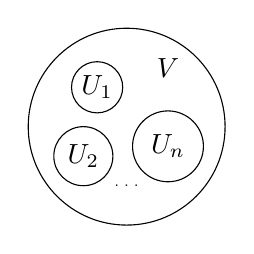
\begin{tikzpicture}[scale=0.25]
 \draw (0,0) circle (5);
 \draw (-1.5,2) circle(1.3) node {$U_1$};
 \draw (-2.2,-1.5) circle (1.5) node {$U_2$};
 \draw (0, -3) node {\tiny$\dots$};
 \draw (2.1,-1) circle (1.8) node {$U_n$};
 \draw (2.1, 3) node {$V$};
 \end{tikzpicture}
 \end{minipage}
\hspace{0.7cm} $\rightsquigarrow$ \hspace{0.5cm}
 \begin{minipage}[c]{8cm}
$\cF(U_1)\otimes\dots\otimes\cF(U_n)\xto{m_V^{U_1,\ldots,U_n}}\cF(V),$
 \end{minipage}
\end{center}

\item The maps are compatible in the obvious way, so that if $U_{i,1}\sqcup\cdots\sqcup U_{i,n_i}\subseteq V_i$ and $V_1\sqcup\cdots\sqcup V_k\subseteq W$, the following diagram commutes.
\begin{center}
\begin{tikzcd}[column sep=small]
{\bigotimes}^{k}_{i=1}{\bigotimes}^{n_i}_{j=1}\cF(U_j) \arrow{dr} \arrow{rr} &   &{\bigotimes}^k_{i=1}\cF(V_i) \arrow{dl}\\
&\cF(W)  &
\end{tikzcd}
\end{center}
\end{itemize}
\end{dfn}

For an explicit example of the associativity, consider the following picture.
\begin{center}
\hspace{-1cm}
\begin{minipage}{3cm}
{\tiny
\begin{center}
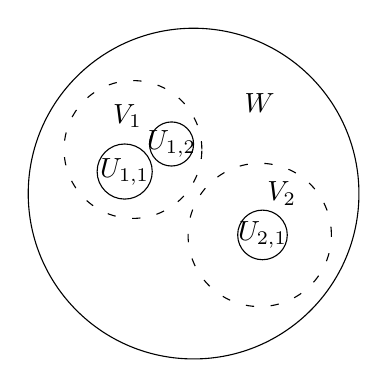
\begin{tikzpicture}[scale=0.35]
 % big circle:
\draw (0,0) circle (6);
\draw (2.4, 3.3) node {$W$};
 % circle V_1:
\draw [style=loosely dashed] (-2.2,1.6) circle (2.5);
\draw (-2.4, 2.8) node {$V_1$};
 % circle V_2:
\draw [style=loosely dashed] (2.4,-1.5) circle (2.6);
\draw (3.2, 0) node {$V_2$};
 % small circles:
\draw (-2.5, 0.8) circle (1) node {$U_{1,1}$};
\draw (-0.8, 1.8) circle (0.8) node {$U_{1,2}$};
\draw (2.5,-1.5) circle (0.9) node {$U_{2,1}$};
%\draw (2.9, -2.1) circle (1.1) node {$U_{2,2}$};
\end{tikzpicture}
\end{center}
}
 \end{minipage}
 \hspace{1.3cm} $\rightsquigarrow$ \hspace{-0.1cm}
\begin{minipage}{8cm}
\begin{tikzcd}[column sep=small]
\cF(U_{1,1}) \otimes \cF(U_{1,2}) \otimes \cF(U_{2,1}) \arrow{dr} \arrow{r}  & \cF(V_1) \otimes \cF(V_2) \arrow{d}\\
&\cF(W) 
\end{tikzcd}
\end{minipage}

The case of $k=n_1=2$, $n_2 = 1$.
\end{center}

This definition bears analogies to familiar objects in mathematics.
On the one hand, $\cF$ resembles a {\em precosheaf}, which is a functor from opens in $M$ to a category like ${\rm Vect}$ or ${\rm dgVect}$.
(A presheaf is a functor out of the opposite category to opens in~$M$.) 
Here, however, $\cF$ also assign values to disjoint unions of opens, and it uses the tensor product rather than direct sum.
This feature leads to the other analogy: $\cF$ resembles an algebra, as
the multilinear maps look like multiplications.
These maps let us multiply elements from disjoint regions to get an element in a larger region.

%Note that these axioms imply that $\cF(\emptyset)$ is a commutative algebra. 
%We say that $\cF$ is a \emph{unital} prefactorization algebra if $\cF(\emptyset)$ is a unital commutative algebra. In this case, $\cF(U)$ is a pointed cochain complex by the image of the unit $1 \in \cF(\emptyset)$ under the structure map $\cF(\emptyset) \to \cF(U)$. In practice, for our examples, $\cF(\emptyset)$ is $\CC$, $\RR$, $\CC[[\hbar]]$, or $\RR[[\hbar]]$. 

\begin{eg}\label{ex:associativealgebra}
Every associative algebra $A$ defines a prefactorization algebra $\cF_A$ on $\RR$, as follows. To each open interval $(a,b)$, we set $\cF_A( (a,b) ) = A$. To any open set $U = \coprod_j I_j$, where each $I_j$ is an open interval, we set $\cF(U) = \bigotimes_j A$. The structure maps simply arise from the multiplication map for $A$. Figure ~\ref{fig:assasfact} displays the structure of $\cF_A$. Notice the resemblance to the notion of an $E_1$ or $A_\infty$ algebra. 
%(One takes an infinite tensor products of unital algebras, as follows. Given an infinite set $I$, consider the poset of finite subsets of $I$, ordered by inclusion. For each finite subset $J \subset I$, we can take the tensor product $A^J = \bigotimes_{j \in J} A$. For $J \hookrightarrow J'$, we define a map $A^J \to A^{J'}$ by tensoring with the identity $1 \in A$ for every $j \in J' \backslash J$. Then $A^I$ is the colimit over this poset.) 
~\hfill$\Diamond$
\end{eg}

%\begin{figure}
%\begin{center}
% \begin{minipage}{3cm}
% \begin{tikzpicture}[scale=0.75]
% \begin{scope}[line cap=round,ultra thick]
% \draw (-2.5,0) -- (-1.5,0); 
% \draw (-1,0) -- (-0.5,0); 
% \draw (1,0) -- (2,0); 
% \draw[->,semithick] (0,-0.5) -- (0,-1.5);
% \draw (-2.75,-2) -- (-0.25,-2); 
% \draw (0.75,-2) -- (2.5,-2);  
% \draw[->,semithick] (0,-2.5) -- (0,-3.5);
% \draw (-3,-4) -- (3,-4); 
% \end{scope}
% \end{tikzpicture}
% \end{minipage}
%\hspace{2cm} $\rightsquigarrow$ \hspace{0.5cm}
% \begin{minipage}{8cm}
% \begin{tikzcd}[cramped,column sep=tiny]
%a \otimes b \otimes c \arrow[mapsto]{d} & \in & A \otimes A \otimes A \arrow{d} \\
%ab \otimes c \arrow[mapsto]{d} & \in & A \otimes A \arrow{d} \\
%abc  & \in &A 
%\end{tikzcd}
%\end{minipage}
%\end{center}

\begin{figure}
\begin{center}
 \begin{tikzpicture} 
 \begin{scope}[line cap=round,ultra thick]
 \draw (-2.5,1) -- (-1.5,1); 
 \draw (-1,1) -- (-0.5,1); 
 \draw (1,1) -- (2,1); 
 \draw[->,semithick] (0,0.75) -- (0,0.25);
 \draw (-2.75,-0.1) -- (-0.25,-0.1); 
 \draw (0.75,-0.1) -- (2.5,-0.1);  
 \draw[->,semithick] (0,-0.35) -- (0,-0.85);
 \draw (-3,-1.2) -- (3,-1.2); 
 \end{scope}
 
\node at (4,0) {$\rightsquigarrow$ };

\node at (7,0){
\begin{tikzcd}[cramped,column sep=tiny]
a \otimes b \otimes c \arrow[mapsto]{d} & \in & A \otimes A \otimes A \arrow{d} \\
ab \otimes c \arrow[mapsto]{d} & \in & A \otimes A \arrow{d} \\
abc  & \in &A 
\end{tikzcd}
};
\end{tikzpicture}
\end{center}
\caption{The prefactorization algebra $\cF_A$ of an associative algebra $A$}
\label{fig:assasfact}
\end{figure}

\begin{eg}\label{ex:SymOfCosheaf}
Another important example for us is the symmetric algebra of a precosheaf. 
Let $F$ be a precosheaf of vector spaces on a space $X$. 
For example, consider $F = C^\infty_c$ the compactly supported smooth functions on a manifold. The functor $\cF  = \Sym F: U \mapsto \Sym(F(U))$ defines a precosheaf of commutative algebras, but it also a prefactorization algebra. For instance, if $U$ and $V$ are disjoint opens, we see that
\begin{align*}
\cF(U \sqcup V) = \Sym F(U \sqcup V) & \cong \Sym (F(U) \oplus F(V)) \\ & \cong \Sym(F(U)) \otimes \Sym(F(V)) = \cF(U) \otimes \cF(V),
\end{align*}
and these isomorphisms provide the structure maps for $\cF$.~\hfill$\Diamond$
\end{eg}

There is another, more sophisticated way to phrase prefactorization algebras, using the framework of operads.
Associated to each topological space $M$, there is a colored operad $\Disj_M$ such that a prefactorization algebra is an algebra over~$\Disj_M$.
For a discussion, see Chapter 3 of~\cite{CG1};
related ideas are developed in~\cite{AF, LurieHA, Ginot}.

%\subsection{Prefactorization algebras as algebras over an operad}
%\label{sec:disj}
%
%The language of colored operads offers a convenient way to formalize the notion of prefactorization algebra.
%A colored operad is a generalization of the idea of a category, where one allows many-to-one maps, and so the term ``multicategory'' is sometimes used. 
%See \owen{add citations}
%
%\begin{dfn}
%Let $\Disj_M$ denote the following colored operad associated to~$M$: 
%\begin{itemize}
%\item The colors (or objects) consist of all open subsets of $M$. 
%\item For every (possibly empty) finite collection of open sets $\{U_\alpha\}_{\alpha \in A}$ and open set $V$, there is a set of maps $\Disj_M( \{U_\alpha\}_{\alpha \in A} \mcol V)$. If the $U_\alpha$ are pairwise disjoint and all are contained in $V$, then the set of maps is a single point. Otherwise, the set of maps is empty.
%\item The composition of maps is defined in the obvious way. 
%\end{itemize}
%\end{dfn}
%
%\begin{dfn}
%Let $\mc{C}$ be a colored operad. 
%A \emph{prefactorization algebra}  on $M$ taking values in $\mc{C}$ is a map of colored operads from $\Disj_M$ to~$\mc{C}$. 
%\end{dfn}
%
%In other words, a prefactorization algebra \emph{is} an algebra over the colored operad $\Disj_M$.
%Since symmetric monoidal categories are special kinds of multicategories, this definition makes sense for symmetric monoidal categories. 
%
%\begin{rmk} 
%If $\mc{C}$ is a symmetric monoidal category under coproduct, then a precosheaf on $M$ with values in $\mc{C}$ defines a prefactorization algebra valued in $\mc{C}$. 
%Hence, our definition broadens the idea of ``inclusion of open sets leads to inclusion of sections'' by allowing more general monoidal structures to ``combine'' the sections on disjoint open sets.
%~\hfill$\Diamond$ 
%\end{rmk}
%
%Note that if $\cF$ is any prefactorization algebra, then $\cF(\emptyset)$ is a commutative algebra object of $\mc{C}$. 
%
%\begin{dfn}
%We say a prefactorization algebra $\cF$ is \emph{unital} if the commutative algebra $\cF(\emptyset)$ is unital. 
%\end{dfn}
%
%\subsection{Encoding ordinary algebras and modules using prefactorization algebras on $\RR$}
%\label{AssAsFact}
%
%We explained above how an associative algebra provides a prefactorization algebra on the real line. There are, however, prefactorization algebras on $\RR$ that do {\em not} come from associative algebras. Here we will characterize those that do arise from associative algebras.
% 
%\begin{dfn}
%Let $\cF$ be a prefactorization algebra on $\RR$ taking values in the category of vector spaces (without any grading).   
%We say $\cF$ is \emph{locally constant} if the map $\cF(U) \to \cF(V)$ is an isomorphism for any  inclusion of open intervals $U \subset V$. 
%\end{dfn}
%
%It is an illuminating exercise to check that this property ensures a prefactorization algebra encodes an associative algebra.
%
%\begin{lem}\label{locally_constant_is_associative}
%Let $\cF$ be a locally constant, unital prefactorization algebra on $\RR$ taking values in vector spaces. 
%Let $A = \cF(\RR)$. Then $A$ has a natural structure of an associative algebra.  
%\end{lem}
%
%One can got further, however, and also capture modules, essentially by marking the line with points.
%For simplicity, we will continue to work with ordinary vector spaces with the tensor product as symmetric monoidal structure.
%
%Let $A$ and $B$ be associative algebras and $M$ an $A-B$-bimodule, i.e., $M$ is a left $A$-module and a right $B$-module and these structures are compatible in that $(am)b = a(mb)$ for all $a \in A$, $b \in B$, and $m \in M$. 
%We now construct a prefactorization algebra $\cF_M$ on $\RR$ that encodes this bimodule structure. 
%
%Pick a point $p \in \RR$. On the half-line $\{x \in \RR \mid x < p\}$, $\cF_M$ is given by $\cF_A$: to an interval $I = (t_0,t_1)$ with $t_1 <p$, $\cF_M(I) = A$, and the structure map for inclusion of finitely many disjoint intervals into a bigger interval is determined by multiplication in $A$. Likewise, on the half-line $\{x \in \RR \mid p < x\}$, $\cF_M$ is given by $\cF_B$. Intervals containing $p$ are determined, though, by $M$. When we consider an interval $I = (t_0,t_1)$ such that $t_0 < p < t_1$, we set $\cF_M(I)  = M$. The structure maps are also determined by the bimodule structure. For example, given 
%\[
%s_0 < s_1 < t_0 < p < t_1 < u_0 < u_1,
%\]
%we have
%\begin{align*}
%\cF_M((s_0,s_1) \sqcup (t_0, t_1) \sqcup (u_0 , u_1)) 
%&= \cF_M((s_0,s_1)) \ot \cF_M((t_0, t_1)) \ot \cF_M((u_0 , u_1)) \\
%&= A \ot M \ot B
%\end{align*}
%and the inclusion of these three intervals into $(s_0,u_1)$ is the map
%\[
%\begin{array}{ccc}
%\cF_M((s_0,s_1)) \ot \cF_M((t_0, t_1)) \ot \cF_M((u_0 , u_1)) & \to & \cF_M((s_0,u_1)) \\
%a \ot m \ot b & \mapsto & amb
%\end{array}.
%\]
%The definition of a bimodule ensures that we have a prefactorization algebra. See Figure ~\ref{fig:bimodasfact}.
%
%%\begin{figure}
%%\begin{center}
%% \begin{minipage}{3cm}
%% \begin{tikzpicture}[scale=0.75]
%% \begin{scope}[line cap=round,ultra thick]
%% \draw (-2.5,0) -- (-1.5,0); 
%% \draw (-1,0) -- (0.5,0); 
%% \draw[fill=black] (0,0) circle (0.07);
%% \draw (1.5,0) -- (2.5,0); 
%% \draw[->,semithick] (0,-0.5) -- (0,-1.5);
%% \draw (-2.75,-2) -- (0.75,-2); 
%% \draw[fill=black] (0,-2) circle (0.07);
%% \draw (1.25,-2) -- (2.75,-2);  
%% \draw[->,semithick] (0,-2.5) -- (0,-3.5);
%% \draw (-3,-4) -- (3,-4);
%% \draw[fill=black] (0,-4) circle (0.07); 
%% \end{scope}
%% \end{tikzpicture}
%% \end{minipage}
%%\hspace{2cm} $\rightsquigarrow$ \hspace{0.5cm}
%% \begin{minipage}{8cm}
%% \begin{tikzcd}[cramped,column sep=tiny]
%%a \otimes m \otimes b \arrow[mapsto]{d} & \in & A \otimes M \otimes B \arrow{d} \\
%%am \otimes b \arrow[mapsto]{d} & \in & M \otimes B \arrow{d} \\
%%amb  & \in &M 
%%\end{tikzcd}
%%\end{minipage}
%%\end{center}
%%\caption{The prefactorization algebra $\cF_M$ for the $A-B$-bimodule $M$}
%%\label{fig:bimodasfact}
%%\end{figure}
%
%\begin{figure}
%\begin{center}
% \begin{tikzpicture}
% \begin{scope}[line cap=round,ultra thick]
% \draw (-2.5,1) -- (-1.5,1); 
% \draw (-1,1) -- (0.5,1); 
% \draw[fill=black] (0,1) circle (0.07);
% \draw (1.5,1) -- (2.5,1); 
% \draw[->,semithick] (0,0.75) -- (0,0.25);
% \draw (-2.75,-0.1) -- (0.75,-0.1); 
% \draw[fill=black] (0,-0.1) circle (0.07);
% \draw (1.25,-0.1) -- (2.75,-0.1);  
% \draw[->,semithick] (0,-0.35) -- (0,-0.85);
% \draw (-3,-1.2) -- (3,-1.2);
% \draw[fill=black] (0,-1.2) circle (0.07); 
% \end{scope}
%
%\node at (4,0){$\rightsquigarrow$};
%
%\node at (7,0) {
%\begin{tikzcd}[cramped,column sep=tiny]
%a \otimes m \otimes b \arrow[mapsto]{d} & \in & A \otimes M \otimes B \arrow{d} \\
%am \otimes b \arrow[mapsto]{d} & \in & M \otimes B \arrow{d} \\
%amb  & \in &M 
%\end{tikzcd}
%};
%
%\end{tikzpicture}
%\end{center}
%\caption{The prefactorization algebra $\cF_M$ for the $A-B$-bimodule $M$}
%\label{fig:bimodasfact}
%\end{figure}

\subsection{Meet factorization algebras}

We are now in a position to define factorization algebras,
which are prefactorization algebras whose behavior on large open sets is determined by their behavior on small open sets.
To give a precise description, we introduce a Grothendieck topology due to Michael Weiss~\owen{cite  \cite{Weiss} and it is explained nicely and further developed in \cite{BoavidaWeiss}}.

\begin{dfn}
Let $U$ be an open set. A collection of open sets $\mathfrak{U} = \{ U_i \mid i \in I\}$ is a {\em Weiss cover} of $U$ if for any finite collection of points $\{x_1,\ldots,x_k\}$ in $U$, there is an open set $U_i \in \mathfrak{U}$ such that $\{x_1,\ldots,x_k\} \subset U_i$.
\end{dfn}

The Weiss covers define a Grothendieck topology on $\Open(M)$, the poset category of open subsets of a space $M$. We call it the {\em Weiss topology} of~$M$. 
Note that Weiss covers are required to ``know'' about every configuration of finitely many points,
and so they often contain many opens.
For a smooth $n$-manifold $M$, a useful Weiss cover is the collection of open sets in $M$ diffeomorphic to a disjoint union of finitely many copies of the open $n$-disc.
(If one has a metric on the manifold, one can work with unions of ``small'' discs.)


%\begin{rmk}
%A Weiss cover is certainly a cover in the usual sense, but a Weiss cover typically contains an enormous number of opens. It is a kind of ``exponentiation" of the usual notion of cover, because a Weiss cover is well-suited to studying all configuration spaces of finitely many points in $U$. For instance, given a Weiss cover $\mathfrak{U}$ of $U$, the collection 
%\[
%\{ U_i^n \mid i \in I\}
%\]
%provides a cover in the usual sense of $U^n \subset M^n$ for every positive integer~$n$.\hfill$\Diamond$ 
%\end{rmk}
%
%\begin{eg}\label{WeissAsExponential}
%For a smooth $n$-manifold $M$, there are several simple ways to construct a Weiss cover for $M$. One construction is simply to take the collection of open sets in $M$ diffeomorphic to a disjoint union of finitely many copies of the open $n$-disc. Alternatively, the collection of opens $\{ M \setminus q \mcol q \in M\}$ is a Weiss cover of $M$. One can also produce a Weiss cover of a manifold with countably many elements. Fix a Riemannian metric on $M$. Pick a collection of points $\{q_n\in M \mcol n \in \NN\}$ such that the union of the unit ``discs'' $D_1(q_n) = \{ q \in M \mcol \d(q_n,q) < 1\}$ covers $M$. (Such an open may not be homeomorphic to a disc if the injectivity radius of $q_n$ is less than 1.)  Consider the collection of all ``discs'' $\fD = \{ D_{1/m}(q_n) \mcol m \in \NN, n \in \NN\}$.  The collection of all finite, pairwise disjoint union of elements of $\fD$ is a countable Weiss cover.~\hfill $\Diamond$ 
%\end{eg}

Now that we have a notion of cover, we can formulate the local-to-global property for factorization algebras.

\begin{dfn}
A \emph{factorization algebra} is a prefactorization algebra $\cF$ on $M$ with values in a symmetric monoidal category $\cC^\otimes$ that is a cosheaf for the Weiss topology.
\end{dfn}

Being a cosheaf means that for any open set $U \subset M$ and any Weiss cover $\{ U_\alpha\}$ of $U$,
the value of $\cF(U)$ can be reconstructed using the \v{C}ech complex:
\[
\cF(U) \xto{\simeq} \check{C}(\mathfrak{U},\cF).
\]
Replacing cochain complexes with some other category (or $\infty$-category), one needs to take a (homotopy) colimit over the \v{C}ech nerve of the Weiss cover.

As verification that this notion has some real content, let's consider a first, interesting case.
We already explained how to produce a locally constant prefactorization algebra $\cF_A$ on $\RR$ from a dg associative algebra $A$.
We could ask about working on the circle $S^1$ instead of $\RR$.
This construction tells us what to assign to every proper open subset of $S^1$: for instance, to each open interval, we assign $A$.
The \v{C}ech complex should then tell us what to assign to the whole circle.
Remarkably, this construction recovers a well-known invariant: the Hochschild chains ${\rm Hoch}_*(A)$ of~$A$.

\begin{thm}[\owen{citations}]
The prefactorization algebra $\cF_A$ extends to a factorization algebra on $S^1$, and
\[
{\rm Hoch}_\bu(A) \simeq \check{C}(\mathfrak{U},\cF_A)
\]
for any Weiss cover of~$S^1$.
\end{thm}

This theorem tells us that factorization homology can be seen as a generalization of Hochschild homology,
where one simultaneously generalizes the circle to an arbitrary closed manifold and an algebra to a factorization algebra.

%Many examples of factorization algebras satisfy an additional and desirable property,
%which motivates the name ``factorization algebra.''
%
%\begin{dfn}
%A factorization algebra $\cF$ is \emph{multiplicative} if for every pair $U,V$ of disjoint open subsets of $M$, the structure map
%$$
%\cF(U) \otimes \cF(V) \to \cF(U \sqcup V) 
%$$
%is a quasi-isomorphism.
%\end{dfn}

\subsection{How factorization algebras appear in QFT}

%Associative algebras are familiar to every mathematician, but as we have just seen, they reflect and encode one-dimensional geometry.
%It is then natural to ask about higher-dimensional versions of algebra.
%Topologists developed such a systematic generalization, often called $E_n$ algebras or algebras over the little $n$-discs operad,
%which we now describe and relate to prefactorization algebras on~$\RR^n$.
%In relation to the subject of this paper, we mention that $E_n$ algebras arise naturally from $n$-dimensional topological field theories;
%we will soon introduce a holomorphic analog of $E_n$ algebras relevant to holomorphic field theories,
%modeled on the discussion here.
%
%Fix a dimension $n$. 
%Let $D^n(x,r)$ denote the open disc of radius $r$ centered at $x \in \RR^n$,
%and let $D^n$ denote the unit disc~$D^n(0,1)$.
%
%\begin{dfn}
%Let $E_n$ denote the colored operad with a single color $D^n$ and a topological space $E_n(k)$ of maps from $k$ copies of $D^n$ to itself given by configurations of $k$ disjoint discs:
%\[
%E_n(k) = \left\{ \begin{matrix}(x_1, \ldots, x_k) \in (D^n(0,1))^k,\\ (r_1, \ldots, r_k) \in (0,1)^k\end{matrix} \,\bigg|\, \text{\begin{tabular}{c}the discs $D^n(x_i,r_i)$ are pairwise disjoint\\ but each contained in the unit disc $D^n$\end{tabular}}\right\}.
%\]
%\end{dfn}
%
%When $n = 1$, the operad encodes the idea of associative multiplication:
%we get pictures much like those we drew earlier with intervals, 
%except that now we can slide and stretch the intervals because we have a space of operations.
%More accurately, $E_1$ is a model for associative algebras up to homotopy; 
%it is closely related to the $A_\infty$ operad. \owen{Let me check how people compare these.}
%
%For arbitrary $n$, this definition encodes concretely the idea of $n$ directions of multiplication.
%If one fixes a direction, such as a coordinate axis, and works with discs lined up in this direction,
%one sees an $E_1$ structure.
%
%\owen{Add picture? We drew 2d pictures earlier.}
%
%An algebra over this operad is called an {\em $E_n$-algebra}.
%A classic example from topology is given by taking the $n$-fold based loop space
%\[
%\Omega^n_x(X) = \{ \gamma: \overline{D^n} \to X \mcol \gamma(\partial \overline{D^n}) = x\}
%\]
%of a based space $(X,x)$ (i.e., a topological space with a distinguished point) and $\overline{D^n}$ denotes the closed unit $n$-disc.
%Maps that send the boundary of a disc to the base point can be extended naturally to bigger discs: just send the rest of the big disc to the basepoint.
%\owen{Should I spell out the structure of the algebra?}
%Examples include \owen{What to mention?}

Factorization algebras on $\RR^n$ and $E_n$ algebras should be closely related,
as can be seen by drawing pictures of the configurations of discs that control operations.

\begin{dfn}
A factorization algebra $\cF$ on an $n$-manifold $M$ is \emph{locally constant} if for each inclusion of open discs $D \subset D'$, then the map $\cF(D) \to \cF(D')$ is a quasi-isomorphism.
\end{dfn}

For $M = \RR$, we have already discussed how locally constant factorization algebras relate to associative algebras, starting with Example~\ref{ex:associativealgebra}.
Lurie has shown the following vast extension of this example. (See section 5.4.5 of \cite{LurieHA}, particularly Theorem 5.4.5.9.)

\begin{thm}\label{thm:locisen}
There is an equivalence of $(\infty,1)$-categories between $E_n$ algebras and locally constant factorization algebras on~$\RR^n$.  
\end{thm}  

\begin{rmk}
We remark that Lurie and Ayala-Francis uses a different gluing axiom than we do. A careful comparison of the different axioms and a proof of their equivalence (for locally constant factorization algebras) can be found in \cite{Matsuoka}.~\hfill $\Diamond$
\end{rmk}

This perspective suggests that factorization algebras offer a natural generalization to field theories on manifolds, and not just on Euclidean spaces. Indeed \cite{CG1, CG2} provide a systematic relationship between field theories and factorization algebras.
The slogan is 
\begin{quote}
the observables of a field theory living on a manifold $M$ form a factorization algebra on~$M$. 
\end{quote}
To physicists, this claim should not be so surprising:
the Weiss cosheaf condition offers a precise version of the idea that a quantum field theory can be fully encoded by all its $n$-point functions.

To make a mathematical statement, one needs to be precise about what a field theory is.
Here, we will mean the definitions articulated in \cite{CosBook,CG1, CG2}, which encompass the Euclidean versions of many field theories studied in physics and mathematics.
Those books use the Batalin-Vilkovisky (BV) formalism for quantization, a homological method generalizing the BRST approach and widely regarded as the most powerful and general way to quantize gauge theories. 

\begin{thm}
\label{main}
The observables of a classical field theory on $M$ form a factorization algebra $\Obs^{cl}$ that assigns to every open set, a 1-shifted Poisson algebra (i.e., a commutative dg algebra equipped with a Poisson bracket of cohomological degree one). A BV quantization of this theory yields a factorization algebra $\Obs^q$ that is a flat deformation of $\Obs^{cl}$ over~$\RR[[\hbar]]$.
\end{thm}

This theorem provides an elegant interpretation of BV quantization as a kind of deformation quantization. In the setting of mechanics (or one-dimensional field theory, since a particle has a worldline), deformation quantization explains the transition from classical to quantum as deforming the observables from a Poisson algebra to an associative algebra. 
This theorem allows one to interpret quantization of field theories---on manifolds of arbitrary dimension---as a deformation quantization from a 1-shifted Poisson factorization algebra to a plain factorization algebra. 

This theorem is also a key connection between field theories and higher algebras.
\owen{I feel like I should say a little more, but not a lot more. I've commented out some old versions of this.}

%In \cite{CG1}, there are several examples of this formalism in action:
%\begin{itemize}
%\item Basic examples from quantum mechanics, such as the harmonic oscillator, and it is shown how to recover the Weyl algebra and the Hamiltonians from factorization algebras living on~$\RR$. 
%\item Scalar field theory on $\RR^n$, where it is shown how the usual correlation functions are encoded in the factorization algebra on~$\RR^n$ and how canonical quantization appears via pushforward of factorization algebras.
%\item The free $\beta\gamma$ system on $\CC$---a basic example of a chiral conformal field theory---is constructed and its usual vertex algebra is extracted from the factorization algebra.
%\item Abelian Chern-Simons theory, where it is shown how dimensional reduction along a closed surface $\Sigma$ produces the Weyl algebra on the symplectic vector space $H^1(\Sigma)$ and how line operators form a (very simple!) braided monoidal category.
%\end{itemize}
%These examples, while not complicated, exhibit in detail how factorization algebras provide a bridge from action functionals to algebra in a broad sense. 
%
%This formalism has shown its power in a number of nontrivial applications:
%\begin{itemize}
%\item Grady, Li, and Li \cite{GLL} give a direct connection between Fedosov quantization and the factorization algebra of a 1-dimensional field theory.
%%\item Gorbounov, Williams and I \cite{GGW} constructed rigorously a 2-dimensional QFT depending on a Calabi-Yau manifold $X$, known as the curved $\beta\gamma$ system, and showed the factorization algebra recovers the chiral differential operators of~$X$.
%\item Li and Li \cite{LiLi} constructed the topological B-model and show the factorization algebra recovers the expected topological vertex algebra (see \cite{LiVOA} for a deeper treatment).
%\item Costello, Francis, and Gwilliam \cite{CFG} have shown how the factorization algebra of Chern-Simons theory for $\fg$ encodes a quantum group $U_\hbar \fg$ over~$\CC[[\hbar]]$.
%\item Rabinovich \cite{RabAxial} showed how the local index theorem and the axial anomaly are simultaneously captured by quantizing free fermions (associated to Dirac operators). Subsequently, he recovered the Quillen determinant line~\cite{RabDet}.
%\item Costello \cite{CosYangian} introduced a 4-dimensional gauge theory whose factorization algebra recovers the Yangian,
%and subsequently gave extensive applications to quantum integrable systems with Witten and Yamazaki \cite{CWY1,CWY2, CY}.
%\end{itemize}
%There are others, connected with central topics such as mirror symmetry and the AdS/CFT correspondence, 
%and we will discuss holomorphic field theories extensively below.
%
%Thanks to the efforts of people who have adopted this BV/factorization framework,
%we now also understand its connection to many important structural aspects of QFT, 
%such as asymptotic freedom \cite{EWY}, current algebras \cite{GWcurr}, the Anderson-Higgs mechanism \cite{EG}, and the CS/WZW correspondence~\cite{GRW, CosDimGai}.
%In each case this enriched mathematical language offers a new and (we would argue) clarifying point of view.
%In turn, physics offers new vistas or rich applications for mathematicians to explore.

%\subsection{$E_n$ algebras from topological field theories}
%
%Although our focus in this paper is on holomorphic field theories and factorization algebras,
%it might be helpful to describe some motivating results about topological field theories and factorization algebras.
%Elliott and Safronov have \owen{not sure how much to say here, but I'm going to take a stab at writing a synoptic theorem}
%
%If one examines theories like Chern-Simons theory on $\RR^3$ or the Poisson $\sigma$-model on $\RR^2$, 
%one discovers a general format for constructing theories that was formalized by \cite{AKSZ}.
%In a nutshell, the field theory is factored into two parts: 
%the de Rham complex of the source or ``spacetime'' manifold, 
%and a Lie algebra-type object encoding a gauge Lie algebra or a ``target'' for a $\sigma$-model.
%
%\begin{dfn}
%A classical {\em AKSZ-type theory} on $\RR^d$ is a determined by an $L_\infty$-algebra $\fg$ equipped with a cyclic pairing $\langle-,-\rangle$ of degree $3-d$.
%Its {\em equation of motion} is the Maurer-Cartan equation 
%\[
%0 = \d A + \frac{1}{2} [A,A] + \frac{1}{3!}[A,A,A]_3 + \cdots = \sum_{k=1}^\infty \frac{1}{k!} [A, \ldots, A]_k
%\]
%of the $L_\infty$ algebra $\Omega^*(\RR^d) \otimes \fg$ with $k$-ary brackets $[-]_k$.
%The {\em action functional} is the expression
%\[
%S(A) = \int_{\RR^d} \sum_{k=1}^\infty \frac{1}{{k+1}!} \langle A, [A, \ldots, A]_k \rangle
%\]
%\end{dfn}
%
%Ordinary Chern-Simons theory on $\RR^3$ arises from taking $\fg$ to be a semisimple Lie algebra and a choice of invariant pairing.
%In that case, and using $\Tr$ to denote the pairing, the action functional is the familiar
%\[
%S(A) = \int_{\RR^3}  \frac{1}{2}\Tr ( A, \d A ) + \frac{1}{3!} \Tr( A, [A, A])
%\]
%and the equation of motion asks for connections with zero curvature.
%
%Many other theories can be expressed in this style, and we suggest \owen{lots of papers} for examples.
%Elliott and Safronov characterize and exhibit topological twists of supersymmetric theories as AKSZ-type theories.
%
%\begin{thm}[\cite{CG2;ElliottSafronov}]
%For a classical AKSZ-type theory on $\RR^d$, the observables 
%\[
%\Obs^{cl}(U) = \clie^*(\Omega^*(U) \otimes \fg)
%\]
%form a locally constant factorization algebra and hence determine an $E_d$ algebra~$\cA^{cl}$.
%A quantization, if it exists, determines a deformation $\cA^q$ of this $E_d$ algebra.
%
%Given a homotopical trivialization of the action of $SO(d)$, then $\cA^q$ is a framed $E_d$ algebra.
%\end{thm}

\subsubsection{Relating to the Atiyah-Segal approach to TFTs}

Atiyah \cite{AtiTFT} offered a mathematical definition for topological field theories that uses symmetric monoidal functors out of bordism categories.
His approach was inspired by Segal's definition of a conformal field theory \cite{SegCFT},
and these notions have subsequently undergone extensive development.
Notably, Baez and Dolan \cite{BaeDol} suggested and advocated for fully extended TFTs; 
their vision was revisited by Lurie \cite{LurieTFT}, who used modern machinery to provide a roadmap for using fully extended TFTs and for proving the cobordism hypothesis.

An important suggestion from \cite{LurieTFT} is that factorization homology allows one to produce nontrivial examples: 
every $E_d$ algebra provides a fully extended $d$-dimensional framed TFT,
albeit taking values in a higher analogue of the Morita bicategory (which works for the $d=1$ case).
Scheimbauer \cite{Scheim} implemented Lurie's suggestion.

\begin{thm}
For any $E_d$ algebra $A$, the functor
\[
\int_{(-)} A \colon {\rm Bord}^{or}_d \to {\rm Alg}_d
\]
determines a fully extended framed $d$-dimensional field theory with values in a higher Morita $(\infty,d)$-category of $E_d$ algebras.
\end{thm}

In combination with the theorem of Elliott and Safronov, we can connect action functionals --- the physicist's usual description of a field theory --- to Atiyah-Segal functorial field theories.

\begin{cor}
For any Lagrangian field theory satisfying the hypotheses of Theorem~\ref{}, 
there is a fully extended framed $d$-dimensional field theory 
given by $\int_{(-)} \cA^q$ where $\cA^q$ denotes the $E_d$ algebra of quantum observables.
\end{cor}

More generally, given a map of Lie groups $G \to O(d)$ and a compatible $G$-action on the theory, 
a homotopical trivialization of this action on the quantum theory equips $\cA^q$ with the structure of a $G$-framed $E_d$ algebra and, by Lurie's work, a $G$-framed fully extended $d$-dimensional TFT.
It is interesting to ask how these kinds of functorial field theories intertwine with the better-known examples.

In this survey we use factorization algebras to capture the rich algebraic structure of holomorphic field theories,
but these connections with functorial TFTs raise the question of producing functorial holomorphic field theories.

\subsection{Examples of holomorphic factorization algebras}



\subsection{Toric (KK) reduction vs. chiralization}

\owen{revisit this theme, and discuss the "modes" algebra}

\section{Holomorphic $\sigma$-models, higher algebras of differential operators, and higher free field realization}

\owen{We should also discuss how these can reduce to LG B-models, as precursor to the Hori-Tong dualities.}

A sheaf of chiral differential operators is a `chiralization' the familiar sheaf of differential operators on a complex manifold \cite{}.
It is a sheaf of vertex algebras $\CDO_X$ on a complex manifold $X$ which satisfies the property that under the Zhu construction one has an isomorphism of sheaves of associative algebras
\beqn
\text{Zhu}(\CDO_X) \simeq \cD_X
\eeqn
where $\cD_X$ is the sheaf of differential operators. 

Unlike the sheaf of differential operators, one needs to fix additional data in order to define a sheaf of chiral differential operators. 
For a smooth complex manifold $X$, one of the main results of \cite{} is that the obstruction to the existence of such a sheaf is given by
\beqn
\ch_2(\T_X) \in H^{2}(X, \Omega^{2,cl}_X) 
\eeqn
and the space of all such algebras of chiral differential operators is a torsor for the group $H^{1}(X, \Omega^{2,cl}_X)$.
Here $\Omega^{2,cl}_X$ is the sheaf of closed holomorphic two-forms on $X$. 

Locally, on an affine patch in $X$, the vertex algebra $\CDO_X$ is equivalent to $N$-copies of the familiar $\beta\gamma$ vertex algebra, where $N = \dim_\CC(X)$. 
We have seen that there is a natural generalization of the $\beta\gamma$ system to a holomorphic factorization algebra in any dimension. 

\begin{dfn}\label{dfn:cdo}
A {\em sheaf of $n$-CDOs} on a manifold $X$ (of complex dimension $N$) is a sheaf of $n$-dimensional holomorphically translation invariant factorization algebras whose restriction to any $n$-disc is equivalent to the $n$-dimensional $\beta\gamma$ system (with target $\CC^N$). 
\end{dfn}

\begin{thm}\label{thm:cdo}
Suppose $X$ is a complex manifold satisfying 
\[
{\rm ch}_{n+1} (\T_X) = 0 \in H^{n+1} \big(X , \Omega^{n+1,cl}_X\big).
\]
Then, the set of equivalence classes of higher dimensional CDO's on $X$ is a torsor for the group $H^n \big(X , \Omega^{n+1, cl}_X\big)$. 
If ${\rm ch}_{n+1}(\T_X) \ne 0$ then there does not exist a sheaf of higher CDO's on $X$. 
\end{thm}

Anticipated by Witten, and proved in \cite{GGW}, the sheaf of chiral differential operators is given by the algebra of local operators of a familiar chiral CFT: the $\beta\gamma$ system of maps $\CC \to X$.
In this note, we have described a higher dimensional analog of this system as a holomorphic $\sigma$-model of maps $\CC^n \to X$. 
We have already met the higher dimensional $\beta\gamma$ system on $\CC^n$.
This is an $n$-dimensional holomorphic system described by an $n$-dimensional translation invariant factorization algebra.
In part, the fields of this system constituted a holomorphic map $\gamma \colon \CC^n \to \CC^N$ together with its conjugate field $\beta$. ''

We can reformulate this theorem to stress the role of the higher dimensional holomorphic OPE. 
An alternative to Definition \ref{dfn:cdo} would be to first take the cohomology of the state space of the $\beta\gamma$ system to obtain the structure of a holomorphic $\PP_n$ algebra.
Then, one can define a sheaf of higher CDO's as a sheaf of holomorphic $\PP_n$ algebras which is locally of the form \eqref{eqn:bgope}. 
Theorem \ref{thm:cdo} still applies to show that a necessary condition for such a sheaf to exist is the vanishing of the $(n+1)$ component of the Chern character of $X$. 
The global sections of such a sheaf will give rise to a single holomorphic $\PP_n$ algebra. 


Let's unravel this approach in the case $n=2$. 
Label the local coordinate on the target by $\{w^i\}_{i=1,\ldots,N}$. 

The cohomology of the state space of the $2$-dimensional $\beta\gamma$ system is a graded polynomial algebra of the form
%\[
%\CC\big[\partial_{z_i}^{\bu \geq 0} \gamma, \partial^{\bu\geq 0}_{z_i} \beta \big]
%\]
\[
\CC\bigg[\gamma^i[k,\ell] \; , \; \beta_j [k,\ell] \bigg]_{k,\ell \geq 0} .
\]
For $k,\ell \geq 0$ and $i,j=1,\ldots N$ the generator $\gamma^i[k,\ell]$ is of cohomological degree zero and the generator $\beta_j[k,\ell]$ is of cohomological degree $1$.

The higher OPEs $\{\gamma^i[k,\ell], \gamma^j [p,q]\}^{r,s} = 0$, $\{\beta^i[k,\ell], \beta^j [p,q]\}^{r,s} = 0$ all vanish. 
There is a nontrivial higher OPE between $\gamma^i$ and $\beta_j$, the simplest of such reads
\[
\big\{\gamma^i[0,0] , \beta_j[-1,-1] \big\}[r,s] = \delta_{r,0} \delta_{s,0} .
\]
In general, 
\beqn\label{eqn:bgope}
\big\{\gamma^i[k,\ell] , \beta_j[p-1,q-1] \big\}[r,s] = \delta_{r,k+p} \delta_{s,\ell+q} .
\eeqn

\subsubsection{Global sections, an example}

We give a concrete description of 2-CDO's on the manifold $X = \PP^1$.
In this case there is a unique sheaf of 2-CDO's that we denote by $2\CDO_{\PP^1}$ (here we are using the holomorphic $\PP_2$ description as the cohomology of the observables of the $\beta\gamma$ system on a $2$-disc).
Consider the standard description of $\PP^1 = U \cup V$ where $U = {\rm Spec}(\CC[\gamma])$ and $V = {\rm Spec}(\CC[\gamma^{-1}])$. 

On $U$, $2\CDO_{\PP^1}(U)$ is the graded polynomial algebra $\CC[\gamma[k,\ell], \beta[p,q]]$. 
On the intersection $U \cup V$ we glue by the transition function
\begin{align*}
\Tilde{\gamma} [k,\ell] & \define \gamma^{-1} [k,\ell] \\
\Tilde{\beta} [p,q] & \define - \sum_{i+j+k=p} \sum_{i'+j'+k'=q} \gamma[i,i'] \gamma[j,j'] \beta[k,k'] + 2 \gamma[p+1, q] + 2 \gamma[p, q+1] .
\end{align*}
\brian{need to fix that I think}

We can gain further insight into the structure of $2\CDO_{\PP^1}$ by the following result. 
Classically, the target $\PP^1$ has an obvious geometric symmetry by the Lie algebra $\sl(2)$ which further lifts to a symmetry by the dg Lie algebra $\fa_2 \otimes \sl(2)$. 

\begin{prop}
The graded vector space $H^\bu \big(\PP^1 \; , \; 2 \CDO_{\PP^1}\big)$ is a module for the graded Lie algebra $H^\bu(\sfA_2) \otimes \sl(2)$
\end{prop}

\begin{rmk}
This result is to be contrasted with the case of ordinary CDO's on $\PP^1$. 
Classically, the one-dimensional $\beta\gamma$ system of maps $\CC \to \PP^1$ has a symmetry by the current algebra $\sfA_1 \otimes \sl(2) = \sl(2)[z,z^{-1}]$. 
At the quantum level, the global sections of ordinary CDO's over $\PP^1$ is a representation for affine Kac--Moody algebra $\Hat{\sl}_2$ at the {\em critical level} \cite[Theorem 5.7]{MSV}. 
In fact, it is isomorphic to a direct sum of two copies of the vacuum representation at the critical level.
This proposition shows that the classical $\sl(2)$-valued $S^3$-currents of global sections of 2-CDO's on $\PP^1$ acquire no such central extension. 
\end{rmk}

Instead of $\PP^1$ let's consider $\PP^2$ thought of as the Grassmannian of lines in $\CC^3$. 
Since $\ch_3(\T_{\PP^2})$ is trivial
the $\beta\gamma$ system of maps $\CC^2 \to \PP^2$ exists at the quantum level and we get a sheaf of 2-CDO's that we denote $2\CDO_{\PP^2}$. \footnote{The sheaf of ordinary CDO's is {\em not defined} on $\PP^2$.} 

The classical $\beta\gamma$ system has, as a symmetry algebra, the $\sl(3)$-valued $S^3$ currents $\sfA_2 \otimes \sl(3)$. 
This is {\em not} a symmetry at the quantum level, rather a {\em higher dimensional Kac--Moody algebra} acts instead.

Let $\theta \in {\rm Sym}^3(\sl(3))$ denote the invariant polynomial $(A,B,C) \mapsto {\rm tr}(ABC)$, where the trace is computed in the {\em defining} representation.
Given $\theta$ we define, as in Section \ref{sec:KM}, the $2$-dimensional Kac--Moody algebra as the $L_\infty$ algebra central extension
\[
0 \to \CC K \to \Hat{\sl(3)}_{2,\theta} \to \sfA_2 \otimes \sl(3) \to 0 .
\]

\begin{prop}
The graded vector space $H^\bu \big(\PP^2 \; , \; 2 \CDO_{\PP^2}\big)$ is a module for the $L_\infty$ algebra $\Hat{\sl(3)}_{2, \theta}$ whereby the central element $K$ acts by multiplication by some nonzero scalar. 
\end{prop}


\subsubsection{Chiralization of the B-model}

In a precise sense, one can view the higher dimensional $\beta\gamma$ system as a holomorphic refinement of a familiar algebra in topological field theory.

\begin{prop}
Let $X$ be a complex manifold with ${\rm ch}_{3}(\T_X) = 0$ and let $2\CDO_X$ be a sheaf of $2$-CDO's on $X$. 
There is an equivalence of sheaves on $X$
\[
{\rm Zhu}_{\EE_2} \big(2\CDO_X) \simeq {\rm PV}^{\bu}_X \define \bigoplus_{i\geq 0} {\rm PV}^i_X [-i] .
\]
Furthermore, the underlying $\PP_2$-structure of the left hand side agrees with the standard Gerstenhaber structure on polyvector fields.
\end{prop}

\begin{rmk}
In this sense, $2\CDO_X$ is a `chiralization' of the sheaf of polyvector fields.
It is distinct from a more standard one coming from the holomorphic twist of the two-dimensional $\cN=(2,2)$ supersymmetric $\sigma$-model.
\end{rmk}

The expert reader will identify the sheaf appearing in the statement of this proposition as local observables of the topological $B$-model on $\RR^2$ with target $X$. 
At the level of quantum field theories, the statement of this proposition is no surprise. 
The key point is that the Zhu algebra (and its $\EE_n$ generalization) is an instance of ``dimensional reduction'' from a holomorphic theory to a topological one. 

On one hand, one considers the $\beta\gamma$ of maps from the two-dimensional complex manifold $\CC^\times \times \CC^\times$ with target manifold $X$:
\[
\T^*[-1] {\rm Map}\left(\CC_\dbar^\times \times \CC_\dbar^\times , X\right) \; \simeq \; {\rm Map}\left(\CC_\dbar^\times \times \CC_\dbar^\times , \T^*[1] X\right) .
\]
In this identification we have used the obvious Calabi--Yau form on $\CC^\times \times \CC^\times$. 
The dimensional reduction of this mapping space along the `doubled' radial projection $\CC^\times \times \CC^\times \to \RR \times \RR$ is precisely the AKSZ description of the ordinary $B$-model with target $X$
\[
{\rm Map}\left(\RR^2_{\rm dR} , \T^*[1] X\right)
\]
in agreement with the proposition above.


\subsubsection{Homogenous spaces}

Suppose that $N$ is a unipotent subgroup of $G$.
For $j \geq 1$ one has
\[
H^j \left( G / N \, ; \, \Omega^{n+1,cl}_{G/N} \right) \; \simeq \; H_{\rm dR}^{j+n+1} \big(G / N \big)
\]


\section{Vista: Seiberg duality and its consequences}
\label{sec: seiberg}

A major endeavor in theoretical physics is to develop a deep and effective understanding of theories like quantum chromodynamics (QCD), which governs the behavior of quarks and gluons.
One natural approach is to study theories that are close cousins but that are easier to analyze,
and a notable way is to look for theories with the same ingredients but with larger groups of symmetries.
Supersymmetric Yang--Mills theories are quite appealing in this regard,
and there have been remarkable successes in this direction.
A well-known high point is the work of Seiberg and Witten on 4-dimensional $\cN =2$ supersymmetric Yang--Mills theory,
where they explained how confinement could be realized by a version of the Mandelstam-'t Hooft mechanism (i.e., a kind of electromagnetic duality identifies confinement with a Meissner effect).
Their work offered powerful new tools that opened up much subsequent progress,
and even impacted mathematics through the Seiberg-Witten equations (which is related to the topologically twisted versions of $\cN=2$ theory).

The class of supersymmetric theories closest to the Standard Model, however, has only $\cN=1$ supersymmetry.
There too Seiberg offered inspiring and powerful insights about SQCD ($\cN=1$ supersymmetric QCD),
and one of his leading contributions is referred to as {\em Seiberg duality}.
It has had a large impact in theoretical physics \owen{give the citation number on that paper},
but the impact in mathematics is much more muted,
possibly due to the lack of a topological twist for any $\cN=1$ theory.
Such theories do admit {\em holomorphic} twists, however, 
and so we explore here what holomorphic Seiberg duality might mean and what its consequences could be in mathematics.
In our opinion this direction could be quite fruitful and we welcome others to join us in exploring it.

We begin this section by describing the holomorphic twist of $\cN=1$ supersymmetric Yang--Mills theory,
and then we offer a holomorphic version of Seiberg duality, 
initially conjectured by Richard Eager.
We explain our first efforts in this direction and how it offers evidence for the conjecture;
we then refine Eager's version.
We also explain how this duality, when compactified along Riemann surfaces,
should produce equivalences between different kinds of 2-dimensional B-model theories;
these reductions are related to work of Hori and Hori--Tong \owen{citations} and its mathematical development by Ed Segal, \owen{list others}.

\subsection{Holomorphic QCD}

A 4-dimensional $\cN=1$ supersymmetric Yang--Mills theory depends on a choice of compact Lie group $G$, with Lie algebra $\fg$, 
and it lives on  the spacetime $M=\RR^4$.
The field content of the theory~is
\begin{itemize}
\item a {\it vector multiplet} that consists of a gauge field $A \in \Omega^1(M) \otimes \fg $ together with some fermions $\lambda \in C^\infty(M) \otimes \fg$, and
\item a {\it matter multiplet} (often called the chiral multiplet), depending on a choice of a representation $V$ of $\fg$, that consists of a scalar $\phi \in C^\infty(M) \otimes V$ together with some fermions $\psi \in C^\infty(M) \otimes V$. 
Additionally, there is a {\it superpotential} $W \in \cO(V)^\fg$, a $G$-invariant polynomial on~$V$. 
\end{itemize}
We always work with super vector spaces, so a fermion means an element of an odd vector space while a boson means an even element.
Thus, we view a fermion $\lambda$ as living in $\Pi (C^\infty(M) \otimes \fg)$,
where $\Pi$ denotes odd parity.

From hereon we fix a nonzero, square zero supercharge $\cQ$ of the 4-dimensional $\cN=1$ supersymmetry algebra.
This element determines a complex structure on $\RR^4$.
We also use it to twist the supersymmetric theory to produce a holomorphic field theory on $\CC^2$.
This twist also has a ``vector'' part and a ``matter'' part.
This twist of 4-dimensional $\cN=1$ supersymmetric Yang--Mills theory has been analyzed and described in \cite{CosYangian, ESW, SWchar}, within that framework for (primarily perturbative) field theory.

This twist has a moduli-theoretic description that we now sketch;
we call a point in such a moduli space a {\it solution to the equations of motion}. 
(We give later a description in terms of fields and action functionals.)
Let $G_\CC$ denote the complex Lie group associated to $G$,
and let $\fg_\CC$ denotes its complex Lie algebra.
We assume that $\fg_\CC$ is equipped with a non-degenerate symmetric invariant pairing and will freely identify $\fg_\CC$ with its linear dual using this data.

The twisted vector multiplet defines a field theory on any complex surface $X$ often called {\em holomorphic BF theory}. 
It will be convenient for us to assume that $X$ is equipped with a holomorphic volume form that we denote by $\Omega_X$. 
A solution encodes a holomorphic $G_\CC$-bundle $\cP \to X$ (by picking out a $\dbar$-connection on the underlying smooth bundle) and a holomorphic section of the adjoint bundle ${\mathrm ad}(\cP) \to X$.
The moduli space can be expressed as the mapping space ${\rm Map}(X, T^*[1]BG_{\CC})$, as a derived stack.
\brian{got rid of the term `shifted' section. Also, to write theory like this we use a CY structure, which I've now fixed.e}

\def\Sslash{\!\sslash\!}

A twisted matter multiplet also defines a field theory on any complex surface $X$. 
\owen{Is it a cotangent theory? It looks like a twisted cotangent theory.}
\brian{right, $i_{dW}$ is the `twist'.}
The superpotential determines a derived affine scheme: the derived critical locus ${\rm Crit}^d(W)$ \brian{How do you feel about the notation $\RR \text{Crit}(W)$?}, which can be modeled as the spectrum of the dg algebra given by polyvector fields $PV(V)$ on $V$ with differential $\iota_{\d W}$.
(It is the Koszul complex associated to the Jacobi ring of $W$.)
This description makes manifest an odd symplectic structure on ${\rm Crit}^d(W)$,
as polyvector fields are an odd Poisson algebra via the Schouten bracket.
%As a dg space, the ring of functions of the derived critical locus is $\cO(\T^* [-1] V)$ equipped with the differential $\iota_{\d W}$. 
By itself (i.e., before coupling to a gauge theory) the twisted matter multiplet corresponds to the mapping space ${\rm Map}(X, {\rm Crit}^d(W))$.\footnote{Notice that AKSZ formalism equips this mapping space with a $1$-shifted symplectic structure as opposed to the desired $(-1)$-shifted symplectic structure.
Hereon we totalize all gradings to $\ZZ/2$.}

Since $W$ is $G_\CC$-invariant, the critical locus has a residual Hamiltonian $G_\CC$-action. 
There is a version of Hamiltonian reduction for odd symplectic manifolds \cite{Pavel, Kevin, who else},
which we denote by ${\rm Crit}(W) \Sslash G_\CC$. 
\owen{I'm not sure we even need this.} \brian{Probably if we want to cite a model for it, I think its fine to list the references here though.}
%As a dg space, the ring of functions is $\clie^\bu\big(\fg , \cO(\fg^* \oplus \Pi \T^* V) \big)$ where the differential is the Chevalley--Eilenberg differential plus $\iota_{\d W}$. 
The holomorphic twist of a theory with both vector and matter multiplets then corresponds to the  derived mapping space
\[
{\rm Map}(X , {\rm Crit}^d(W) \Sslash G_\CC), 
\]
which comes equipped with an odd symplectic structure. 
\owen{Should there also be a factor involving the $B$-fields of the BF gauge theory?}
\brian{That's already in this hamiltonian reduction. 
If $V$ is $(-1)$ shifted symplectic then I think the tangent space of $V \Sslash G$ should be
\beqn
\lie{g}[1] \oplus V \oplus \lie{g}^*[-2] .
\eeqn
Since we're forgetting to $\ZZ/2$ this is just $\Pi \lie{g} \oplus (V \oplus \lie{g})$.
}

We wish to study a holomorphic analog of supersymmetric chromodynamics.
We will call the relevant theory {\it QCD}, following convention, even though it is classical and not yet quantum.
We will specialize $G = SU(N)$ and so $G_\CC = SL(N)$.
The matter fields will consist of two types: quarks and antiquarks.
Let $\underline{N}$ denote the {\em fundamental} (or defining) representation of $SL(N)$,
so $\underline{N} = \CC^N$ with its natural left action.
\owen{That's kind of crappy notation. Let's discuss.}

%All of the holomorphic theories we consider below will be special cases of this gauged linear mapping space with $X = \CC^2$. 
%We slightly refine notation and associate a holomorphic theory $\cT(G, V, Z, W)$ on $\CC^2$ associated to the following data:
%\begin{itemize}
%\item a Lie group $G$, this is the gauge group. 
%Its complexified Lie algebra is $\fg = {\rm Lie}_\CC (G)$;
%\item a complex $G$-representation $V$, this is where the `chiral quark matter' lives;
%\item a complex vector space $Z$ where the `mesons' live.
%This is not acted upon by the group $G$. 
%\item a polynomial $W \in {\rm Sym}(V \oplus \Bar{V} \oplus Z)$.
%\end{itemize}

\begin{dfn}
A {\em holomorphic QCD theory} with $N$ {\em colors} and $F$ {\em flavors} is the holomorphic field theory on $\CC^2$ where
\begin{itemize}
\item the gauge fields are those of holomorphic BF theory valued in $\sl(N)$, whose fields are
\[
A \in \Omega^{0,\bu}(\CC^2 , \sl(N))[1] \quad\text{and}\quad B \in \Omega^{2,\bu}(\CC^2, \sl(N)^*);
\]
\item the ``quarks'' are fields of a holomorphic $\beta\gamma$ system valued in 
\[
V_Q = \Hom(\CC^F, \underline{N}) \cong \underline{N}^{\oplus F} \cong \CC^{NF},
\] 
whose fields are
\[
Q \in \Omega^{0,\bu}(\CC^2 , V_Q) \quad\text{and}\quad R \in \Omega^{2,\bu}(\CC^2 , V_Q^*)[1];
\]
\item the ``antiquarks'' are fields of a holomorphic $\beta\gamma$ system valued in the dual representation 
\[
V^*_Q \cong \Hom(\underline{N}, \CC^F) \cong (\underline{N}^*)^{\oplus F} \cong \CC^{NF}, 
\]
whose fields are
\[
Q^\dag \in \Omega^{0,\bu}(\CC^2 , V^*_Q) \quad\text{and}\quad R^\dag \in \Omega^{2,\bu}(\CC^2 , V_Q) [1].
\]
\end{itemize}
(The superscript $\dag$ does not mean we apply an operation to $Q$ or $R$; 
it is simply to remind us that these fields are the ``antiparticles''.)

The action functional is
\[
S_{QCD} = \int B\, F^{0,2}_A + \int R \,\dbar_A Q + \int r \,\dbar_A q,
\]
where $\dbar_A = \dbar + A$ is the covariant $\dbar$-operator.
\owen{Should we make explicit how we're using the evaluation pairing on fields and their ``conjugates''? Or do we explain that in our review of BF theories?}
%We will denote this theory by $\cT(N,F)$.
\footnote{Although this perturbative theory only depends on the Lie algebra of $G$, the group structure will be relevant when we discuss local operators and moduli of vacua.} 
\end{dfn}

To formulate Seiberg duality, we will need to allow auxiliary matter fields that we call ``mesons.''

\begin{dfn}
A holomorphic QCD theory {\em with mesons}
%, denoted $\cT(N,F, V_M, W)$, 
is a holomorphic QCD with $N$ colors and $F$ flavors along with {\em meson fields}, which form a $\beta\gamma$ system valued in the vector space $V_M$, which we denote by
\[
\mu \in \Omega^{0,\bu}(\CC^2 , V_M) \quad\text{and}\quad \nu \in \Omega^{2,\bu}(\CC^2 , V_M^*) [1] .
\]
The action functional is
\[
S_{QCDwM} = S_{QCD} + \int \nu \,\dbar \mu + \int \d^2 z \; W(Q, \Tilde{Q}, \mu) .
\] 
Notice that to write down the superpotential term we are utilizing the holomorphic volume form $\Omega_X = \d^2 z$. 
\end{dfn}

Note that the fields $\mu$ are ``uncharged,'' i.e., $SL(N)$ acts trivially on $V_M$.
The only coupling that the meson $\mu$ has to the other fields is through the superpotential~$W$. 

\begin{rmk}
This theory is only $\ZZ/2$-graded, so all fields are considered merely as even or odd.
For instance the component of the gauge field $A^{0,1}$ is even while the component of the matter field $Q^{0,1}$ is odd. 
Only when $W = 0$ can one lift the theory to a $\ZZ$-grading.
\end{rmk}

\subsection{A first pass at Seiberg duality}

Our long-term goal is to show that two special cases of holomorphic QCD are {\em dual}.
The notion of duality can refer to several kinds of relationships,
but loosely speaking it means that some aspects of the two theories are equivalent under correspondence.
We will postpone saying anything precise till we have some terminology in place.

%We focus on the gauge group $G = \SU(N)$, and consider a class of holomorphic QCD theories associated to particular choices of representations and superpotential. 
%Following physics terminology, we will refer to the defining $N$-dimensional representation $\CC^N$ of $\SU(N)$ as the {\em fundamental} representation. 
%Also, let $N_c, N_f$ denote integers where $N_f \geq N_c \geq 2$.
%Also, let $N_{\rm mes} \geq 0$ be some integer.  
%{\em Type A} holomorphic QCD is 
%\[
%\cT_{A} (N_c, N_f, N_{\rm mes},W) = \cT\left(G = \SU(N_c) \, , \, V = (\CC^{N_c})^{\oplus N_f} \, , \, Z = \CC^{\oplus N_{\rm mes}} \, , \, W\right) .
%\]

There will be two theories. 
We call one side {\em electric} and the other {\em magnetic}.

\begin{dfn}
Fix a positive integer $F$, for flavor, and fix integers $N$ and $\check{N}$ such that $F = N + \check{N}$ and $F \geq N, \check{N} \geq 2$.

The {\em electric theory} is the holomorphic QCD with $N$ colors and $F$ flavors, {\em without} mesons.
We denote it by~$\cT_{\sfE}(F, N)$.
We use $A, B, Q, R, Q^\dag$, and $R^\dag$ for the fields.

The {\em magnetic theory} $\cT_{\sfM}(F, \check{N})$ is the holomorphic QCD with $\check{N}$ colors and $F$ flavors, but with mesons $\check{\mu}$ where $$V_{\check{M}} = \End(\CC^F) \cong \CC^{\oplus F^2}$$
(and $\check{L}$ for the partner field to $\check{M}$).
We use $\check{A}, \check{B}, \check{Q}, \check{R}, \check{Q}^\dag$, and $\check{R}^\dag$ for the other fields.
The superpotential is $$\check{W} =  \Tr(\check{Q}^\dag \check{\mu}  \check{Q}),$$
where we compose the linear maps before tracing over~$V_{\check{N}}$.
\owen{Please double-check that formula.}
\end{dfn}


Note that the lower bound on $N$ and $\check{N}$ is simply to ensure that we have nontrivial gauge groups.

%In this case the auxiliary vector space $Z$ is nontrivial (but transforms trivially under the gauge group as in the definition). 
%Our notation is $q,\Tilde{q}$ for elements of the vector spaces $V, \Bar{V}$ and $m\in Z$.
%The magnetic theory is
%\[
%\cT_{\sfM} (N_c, N_f) \define \cT\big(\SU(N_f - N_c) \, , \, (\CC^{N_f - N_c})^{\oplus N_f} \, , \, \CC^{\oplus N^2_f} \, , \, W = m q \Tilde{q} \big)
%\]
%In the definition of $W = m q \Tilde{q}$ we are using the natural contractions which we can describe explicitly as follows.
%Choose a basis $\{q_a^i\}$ for $V = (\CC^{N_f - N_c})^{\oplus N_f}$, $a = 1,\ldots, N_f - N_c$, $i=1,\ldots N_f$ and a dual basis $\{\Tilde{q}_i^a\}$ for $\Bar{V}$.
%Also, let $\{m_i^j\}$ be a basis for $\CC^{\oplus N_f^2}$. 
%Then the cubic polynomial $W$ is
%\[
%W = \sum_{i,j,a} m^i_j q_i^a \Tilde{q}^i_a .
%\]

Seiberg duality states how certain ``electric'' and ``magnetic'' versions of SQCD should be equivalent.
The electric and magnetic holomorphic QCDs are precisely the holomorphic twists of those that appear in Seiberg duality,
and so Richard Eager suggested that Seiberg duality should survive after taking the holomorphic twist.

\begin{conj}[\cite{Eager}]
Let $F = N + \check{N}$ and $F \geq N, \check{N} \geq 2$.
Construct a quantization of the theories $\cT_{\sfE}(F,N)$ and $\cT_{\sfM}(F,\check{N})$.
There is an equivalence of 2-dimensional holomorphic factorization algebras
\[
\Obs_{\sfE} \simeq \Obs_{\sfM}  
\]
where these are the observables of the electric and magnetic theories, respectively.
\end{conj}

\owen{Do we want $F > N+1$? The physicists break things into several cases. In particular, I think the moduli is unchanged under quantization only if $F$ is big enough relative to $N$ and $\check{N}$.}

\begin{rmk}
The statement is an equivalence of factorization algebras valued in $\ZZ/2$-graded cochain complexes since the field theories are only $\ZZ/2$-graded.
\end{rmk}

This claim should seem rather surprising.
In many ways these theories look, on their face, like very different theories:
the gauge groups $SL(N)$ and $SL(\check{N})$ are (usually) different, and
one side has mesons and the other does not.
Of course, relating quite different theories also makes the conjecture powerful.

One appealing aspect of Eager's conjecture is that it is mathematically precise:
duality would mean giving an equivalence of factorization algebras.
It is analogous to claiming that two vertex algebras are equivalent,
such as in the well-known boson-fermion correspondence or in the correspondence between the chiral rings of the A- and B-models of mirror symmetry.
In this sense it is a target at which a mathematician can aim,
rather than the more amorphous statements of duality that one often finds in the physics literature.
In that literature, however, there is guidance on what map of factorization algebras provides the equivalence,
which we describe in the next section.

In general, Eager's suggestion opens up a fascinating vein of inquiry:
\begin{quote}
how do physical results about supersymmetric gauge theories behave under twisting to holomorphic or topological theories?
\end{quote}
We have found, so far, that these results often admit clean mathematical formulations and that the holomorphic (or topological) twists involve constructions of natural interest in geometry and representation theory.
In \cite{EGW} we and Chris Elliott explored twists of $\cN=4$ supersymmetric Yang--Mills theory,
provided their quantizations, and began analyzing their factorization algebras.
Following Eager, we can ask about the twisted versions of S-duality and how to provide those conjectured equivalences.
\owen{This should be rephrased, and we should mention more people, like Philsang and Surya. We can mention pre-S-duality things (like our work and the EY stuff) and S-duality stuff.}

\begin{rmk}
Our discussion here is ahistorical.
Witten initiated this vein of research for topological twists \cite{},
and Costello pushed it for holomorphic twists, particularly in the setting of holography \cite{}.
Eager's suggestion was a natural variation on this theme but it (seems to) involve physical ideas and methods that have not (yet) played a large role in Costello's program.
\owen{Add a remark (?) about Kevin and Si's work on twisted holography and other related directions.}
\end{rmk}

\subsection{Evidence for holomorphic Seiberg duality}

We now turn to examining evidence for the conjecture, which will, in turn, allow us to refine it.
The first piece of evidence involves the classical field theories:
\begin{enumerate}
\item[(1)] Each theory has a moduli space of vacua, and there is a natural isomorphism between the spaces for theories dual according to the conjecture.
\end{enumerate}
This map determines a map of factorization algebras of classical observables,
and it should deform to the map between the factorization algebras for the quantum theories.
(There are some interesting geometric subtleties --- about stacks versus their affinizations --- that we discuss below.)

As we discuss in a moment, holomorphic QCD can be quantized using the techniques of \cite{BW work}.
There are then two further pieces of evidence when these quantum theories are examined:
\begin{enumerate}
\item[(2)] There are {\em flavor} symmetries by $SL(F)$ that act on the quarks and antiquarks of each theory, 
and these can be matched under the duality. 
For the classical holomorphic theories, these symmetries enhance to an action of holomorphic $\sl(F)$-valued functions on the quark and antiquark fields.
Under quantization, these have isomorphic anomalies.
\item[(3)] There are {\em spacetime} symmetries that act on each theory, notably isometries, 
and on the classical holomorphic theories, these enhance to an action of holomorphic vector fields. Under quantization, these have isomorphic anomalies.
\end{enumerate}
This triple of evidence is analogous (and sometimes stronger) than results for Seiberg duality for SQCD. 
We now turn to fleshing out these assertions.

\subsubsection{Moduli of vacua and quantization}

It is fruitful, and standard in physics, to identify the simplest solutions to the equations of motion for a theory.
Here that means a solution that is translation-invariant on $\CC^2$ (i.e., a constant solution),
and we call such a solution a {\em classical vacuum}.
Thus each theory has an associated {\em moduli space of classical vacua},
which we describe in the next subsection.
Each vacuum determines a perturbative field theory that one could try to quantize,
and we have shown the following.
(Many arguments are close cousins of~\cite{EGW}, where we quantize every twist over a moduli of vacua of the $\cN=4$ supersymmetric Yang--Mills theory.)

\begin{thm}
Both $\cT_{\sfE}(F,N)$ and $\cT_{\sfM}(F, \check{N})$ exist at the quantum level for any choice of classical vacuum. 
That is, the anomaly to a perturbative BV quantization vanishes.
In fact, the quantization is one-loop exact. 
\end{thm}

It is common in physics to study field theories defined on the spacetime $\RR^n$.
As the underlying spacetime $\RR^n$ is a group under addition (i.e., it is the translation group),
it is natural to ask for field theories with an action by translations.
That is, since the fields are sections of a fiber bundle over $\RR^n$,
one can ask for an equivariant fiber bundle and ask for the equations of motion (or action functional) to be equivariant under translations.
In practice, physicists often work with field theories whose equations of motion are differential equations with constant coefficients.
(Nearly all the examples we've discussed in this survey satisfy this condition.)

Now such a field theory $\cT$ on $\RR^n$ has a space of solutions $\Sol_\cT(\RR^n)$ to its equations of motion.
A {\em classical vacuum} for the theory is a solution that is translation-invariant,
i.e., a constant solution.
As the solutions $\Sol(\RR^n)$ is a derived stack (at least if you adhere to the perspective we've advocated here), there is a derived stack of classical vacua
\[
\cM_{\rm vac}(\cT) = \Sol_\cT(\RR^n)^{\RR^n}
\]
given by the substack of constant solutions.
We call it the {\em moduli stack of classical vacua} for the theory~$\cT$.

Many stacks of interest to geometers and representation theorists appear naturally from holomorphic field theories.
For example, the holomorphic $\sigma$-model from $\CC^d$ into a target complex manifold $X$ has
\[
\cM_{\rm vac} \cong T^*[1-d]X.
\]
(If we consider the underlying underived stack, it is just $X$, unless $d = 1$.)
For supersymmetric gauge theories, the moduli stack of the holomorphic twist has the form
\[
\cM_{\rm vac} \cong [V/G]
\]
where $V$ is a (graded) $G$-representation and $[V/G]$ denotes the quotient stack.
The factor $V$ depends on the non-gauge fields (i.e., matter multiplets), which are sections of some associated vector bundle;
the quotient by $G$ arises from the gauge transformation.
For example, pure $\cN =1$ holomorphic Yang-Mills theory for group $G$ (i.e., the vector multiplet) has
\[
\cM_{\rm vac} \cong \fg^*/G,
\]
the coadjoint quotient stack of the group.
(We are working in a $\ZZ/2$-graded world here.)
Using the invariant pairing on $\fg$ we can further identify this with the adjoint quotient stack~$\fg / G$. 
For general supersymmetric field theories, which involve both a $\sigma$-model and gauge fields, the holomorphic twist has a moduli stack of classical vacua of the form
\[
\cM_{\rm vac} \cong [X/G]
\]
where $X$ is a derived stack with a $G$-action and $[X/G]$ denotes the quotient stack.

In studying questions about the classical vacua of supersymmetric field theories, however, physicists have not typically worked with the {\em stack}.
Instead, they have worked with a GIT quotient.
For instance, in the setting of a gauge theory with moduli stack of classical vacua $[V/G]$, it means they work with 
\brian{I don't like this notation, its confusing since it looks like symplectic reduction which has already appeared. 
What about $[V/G]$?} \owen{I'm happy to do that, but symplectic reduction is the GIT quotient.}
\[
V\Sslash G = \Spec(\cO(V)^G),
\]
the scheme whose ring of functions are the $G$-invariant functions on the representation~$V$.
This affine scheme is known as the {\em affinization} of the stack $V/G$, as it is the best affine approximation to the stack (i.e., apply the left adjoint to the inclusion of affine schemes among stacks).
We will call this GIT quotient the moduli {\em space} of classical vacua and denote it by~$M_{\rm vac}(\cT)$.
(Note that the font of M changes between stack and space.)

\begin{rmk}
In practice physicists work ordinary schemes (i.e., without any derived directions), 
although one can also study the derived affine scheme that is the best approximation to a derived stack.
Below we will always provide an ordinary scheme as the moduli {\em space}.
\end{rmk}

It is familiar to geometers that this affinization forgets interesting information about the stack because an invariant function must be constant on the closure of any orbit.
Thus, the canonical map
\[
[V/G] \to V\Sslash G
\]
often collapses orbits together.
An important example, pertinent to $\cN =1$ super Yang-Mills theory, is the adjoint quotient $[\gl_N/ GL_N]$, whose affinization is
\[
\gl_N \Sslash GL_N \cong \CC^N,
\]
by the Chevalley restriction theorem $\cO(\gl_N)^{\GL_N} \cong \cO(\frak{h})^{S_N}$ where $\frak{h}$ denotes the maximal torus.
(The rightmost algebra is symmetric polynomials.)
The canonical map here records the characteristic polynomial of a matrix and hence only knows its generalized eigenvalues and not its Jordan decomposition.
In other words, the canonical map collapses together Jordan blocks with the same diagonal entries.
For this reason, it loses details about the classical vacua remembered by the stack quotient.

\begin{rmk}
The physicists' focus on the moduli space is not unreasonable:
one must make measurements --- i.e., evaluate functions --- to identify the state of a physical system.
The moduli space captures what can be seen by measurements (notably here, the ``vacuum expectation values'' of different vacua).
In other words, the possible classical states --- viewed as suitable linear functionals on the algebra of observables --- are parametrized by the underlying affine scheme of the derived moduli stack.
On the other hand, the moduli stack knows each orbit, which provides a distinct solution to the equations of motion,
and hence records much more about the classical theory; 
the space cannot distinguish between some vacua because it collapses orbits.
Moreover, the stack encodes much more data about the theory near each vacuum.
For instance, it remembers ``enhanced symmetries'' (such as the residual gauge fields) at each vacuum.
\end{rmk}

For the holomorphic QCD theory with $F$ flavors and $N$ colors (without mesons), 
the moduli stack of classical vacua is 
\[
\cM_{\rm vac}(F,N) \cong T^*[1] \left(V_Q \oplus V_Q^*/SL(N)\right).
\]
By contrast the moduli space $M_{\rm vac}$ is a variety already well-studied in classical algebraic geometry.
Before we jump to the full space, let's examine a simpler case involving just the quarks.
A vacuum for the quark field is an element of $V_Q = \Hom(\CC^F, \CC^N)$,
and it is a classic result of invariant theory that
\[
\Hom(\CC^F, \CC^N)\Sslash SL(N) \cong \widehat{{\rm Gr}(F, N)} \subset \Lambda^N \CC^F
\]
where ${\rm Gr}(F, N)$ denotes the Grassmannian of $N$-planes in $\CC^F$ and the hat indicates we take the affine cone with respect to this standard Pl\"ucker embedding.
For the full problem, we have both quarks and antiquarks, so
\begin{align*}
M_{\rm vac}(F,N) 
&\cong V_Q \oplus V_Q^*\Sslash SL(N) \\
&= \Hom(\CC^F, \CC^N) \oplus \Hom(\CC^N, \CC^F)\Sslash SL(N),
\end{align*}
whose ring of functions is also computed by the fundamental theorems of invariant theory.
Those theorems tell us that the GIT quotient is a closed conical subvariety
\[
M_{\rm vac}(F,N)  \hookrightarrow \Lambda^N \CC^F \times \Lambda^N (\CC^F)^* \times \End(\CC^F)
\]
where a pair of matrices $(X,Y) \in \Hom(\CC^F, \CC^N) \times \Hom(\CC^N, \CC^F)$ goes to $(\Lambda^N X, \Lambda^N Y, YX)$, with $\Lambda^N X$ denoting the wedge product of the rows of $X$ (and of columns for $Y$).
The image thus satisfies both sets of Pl\"ucker relations, the condition that the composite $YX$ has rank at most $N$, and some further relations, given by the Second Fundamental Theorem, such as that the pairing of $\Lambda^N X$ and $\Lambda^N Y$ can be related to $\Lambda^N (YX)$.
(See Chapter 2, Section C of \cite{Weyl}.)
In other words, we have a closed subvariety
\[
M_{\rm vac}(F,N) \hookrightarrow \widehat{{\rm Gr}(F, N)} \times \widehat{{\rm Gr}(F, N)} \times {\rm R}(F,N)
\]
with ${\rm R}(F,N) \subset \End(\CC^F)$ the matrices with rank bounded above by~$N$.
The moduli space for the magnetic theory is a bit more complicated but follows from classical invariant theory as well.

Note that $\check{N} = F-N$, so $\widehat{{\rm Gr}(F, N)} \cong \widehat{{\rm Gr}(F, \check{N})}$,
but ${\rm R}(F,N)$ is not isomorphic to ${\rm R}(F,\check{N})$ except when $N = \check{N}$.
Hence one should not be optimistic that $M_{\rm vac}(F,N) \cong M_{\rm vac}(F,\check{N})$.
To ``fix'' this issue, one might try to slightly modify the dual side, which Seiberg did by adding the meson fields.
Hence the following holds.

\begin{prop}
Seiberg dual theories have isomorphic moduli spaces.
\end{prop}

This relationship, which holds already for the supersymmetric theory before twisting, was one of the original pieces of evidence offered by Seiberg for his duality.
The proof boils down to checking that the mesons and the superpotential on the magnetic side ensure the isomorphism.

\begin{rmk}
In the physics literature this isomorphism is given by explicitly matching gauge-invariant functions, 
which are often called mesons or baryons, 
as they can be identified with the data that identifies such particles.
These meson and baryons are precisely the usual generators of the ring of invariant functions, 
so an isomorphism of generators determines the desired isomorphism of rings. 
One must check that the relations are satisfied;
this requirement explains the superpotential on the magnetic side.
\end{rmk}

We want to point out, however, that {\em the moduli stacks are not isomorphic}.
A quick check is to note that there are orbits with different stabilizer groups.
Consider, for instance, the origin in each vector space.
On the electric side its stabilizer is $SL(N)$ and on the magnetic side it is $SL(\check{N})$.
Thus each theory has a vacuum whose associated perturbative classical theory has no partner on the other side.
Hence Seiberg duality cannot hold at the stack level for the classical theories.

\subsubsection{Flavor symmetries}

The quarks of the electric theory take values in $\Hom(\CC^F, \CC^N)$ and hence have a canonical action of $SL(F)$ by precomposition.
We view each factor $\CC$ inside $\CC^F$ as a different ``flavor'' of quark, so this action mixes flavors.
The antiquarks take values in $\Hom(\CC^N, \CC^F)$ and so have a canonical action of $SL(F)$ by postcomposition.
The action functional is invariant for this action, and thus $SL(F)$ acts naturally on the space of solutions to the equations of motion.
This symmetry is known as {\em flavor} symmetry.
The magnetic theory has an analogous flavor symmetry, where $SL(F)$ acts on the mesons by conjugation.
\owen{Right?}

%We fix some notation for the fields of the electric and magnetic theories. 
%The `flavor' index will be denoted by letters $i,j=1,\ldots, N_f$. 
%
%With respect to a basis for $\CC^{N_f}$ we denote the matter fields of the electric theory as
%\[
%Q^i\; , \; P_i \; , \; \Tilde{Q}_i \; , \; \Tilde{P}^i , \quad i = 1, \ldots, N_f.
%\]
%Each of these fields are Dolbeault forms that are valued in the fundamental $\SU(N_c)$ representation. 
%
%The matter fields of the magnetic theory will be denoted by lower case letters to avoid confusion
%\[
%q^i\; , \; p_i \; , \; \Tilde{q}_i \; , \; \Tilde{p}^i , \quad i = 1, \ldots, N_f.
%\]
%Again, each of these fields are Dolbeault valued but this time they each transform under the fundamental $\SU(N_f-N_c)$ representation. 
%On the magnetic side one also has the `meson' fields $M_{i}^j$, which are scalars under the gauge group.
%
%Holomorphic QCD enjoys a few familiar holomorphic symmetries in the style that we discussed in this note.

For holomorphic QCD theories, the infinitesimal flavor symmetry by the Lie algebra $\sl(F)$ enhances to a symmetry for the infinite-dimensional dg Lie algebra $\Omega^{0,*}(\CC^2, \sl(F))$, 
which we call a $2$-dimensional holomorphic current algebra.
It acts by wedging the forms and applying $\sl(F)$ to the relevant vector space, such as~$\Hom(\CC^F,\CC^N)$.

%The holomorphic background field $\fa = (\fa_i^j) \in \Omega^{0,\bu}(\CC^2 , \sl(N_f))$ naturally couples to both the electric and magnetic theory in the following ways:
%\[
%I^F_\sfE = \int P_j \fa_i^j Q^i , \qquad I^F_\sfM = \int \Tilde{p}_j \sfa_j^i \Tilde{q}^j + \int L^k_j \sfa_i^j M^i_k . 
%\]
%
%This determines a classical symmetry of both sides of the duality by the local Lie algebra $\Omega^{0,\bu}(\CC^2, \sl(N_f))$. 
%In particular, the two state spaces form a module for the $S^3$-current algebra $\sfA_2 \otimes \sl(N_f)$ at the classical level.

A natural question is whether this symmetry persists at the quantum level. 
The answer is {\em yes}, but on both sides of the duality one must use a central extension of the current algebra as an $L_\infty$ algebra.
The extension arises because the symmetry has an anomaly under quantization (on either side of the duality),
and this anomaly is determined by an  invariant cubic polynomial $\theta_\sfE$, $\theta_\sfM$, respectively, on the Lie algebra~$\sl(F)$. 
(In terms of Section \owen{cross ref}, these determine higher Kac--Moody algebras $\Hat{\sl(N_f)}_{2,\theta_{\sfE}}, \Hat{\sl(N_f)}_{2,\theta_{\sfM}}$ when studying the theories on the punctured space~$\CC^2 - \{0\}$.)

\begin{prop}
There is an anomaly at the quantum level for the holomorphic flavor symmetry action for both the electric and magnetic theories,
and they agree: they are labeled by the same cocycle 
\[
\theta_\sfE = \theta_\sfM.
\] 
In particular, the state spaces $\sfV_\sfE, \sfV_\sfM$ are modules for the {\em same} $2$-dimensional higher Kac--Moody algebra $\Hat{\sl(N_f)}_{2,\theta}$.
\end{prop}

An analogous result holds for the flavor symmetry on the antiquarks. 

\begin{proof}[Sketch of proof]
The argument boils down to an explicit presentation of anomalies using the Feynman diagrammatic analysis for holomorphic theories surveyed in Section~\ref{sec:renorm}. 
For this calculation the gauge algebra $\sl(N)$ plays a minimal role. 
The central extension is represented by a series of Feynman diagrams that are wheels with three vertices, each labeled by an element of the current algebra $\sfa \in \Omega^{0,*}(\CC^2, \sl(F))$, which we treat as a background gauge field.
In formulas, we couple the current algebra to both the electric and magnetic theory via interactions
\[
I^F_\sfE = \int (R, \sfa Q)  \qquad\text{and}\qquad I^F_\sfM = \int (\check{R}, \sfa \check{Q}) + \int (\check{\nu}, \sfa \check{\mu}),
\]
where we use parentheses $(-,-)$ to denote the pairings in BF and $\beta\gamma$ theories.

In the electric case there are $N$ such diagrams, with all the internal edges are labeled by $Q-R$ propagators. 
This gives rise to the local anomaly
\beqn\label{eqn:electricflavor}
 \frac{N}{16} \int \op{tr}_{\underline{F}} \left(\sfa \, \partial \sfa \, \partial \sfa\right) 
\eeqn
where $\op{tr}_{\underline{F}}$ denotes the trace in the fundamental $\sl(F)$-representation.

The magnetic theory has two types of wheels whose external edges are labeled by the background field $\sfa$: 
\begin{itemize}
\item[(a)] those with  internal edges labeled by $\check{Q}-\check{R}$ propagators and 
\item[(b)] those will internal edges labeled by $\check{\mu}-\check{\nu}$ propagators. 
\end{itemize}
There are $\check{N} = F - N$ copies of diagram (a), which gives rise to the term
\[
 \frac{\check{N}}{16} \int \op{tr}_{\underline{F}^*} \left(\sfa \, \partial \sfa \, \partial \sfa\right) .
\]
Here, $\op{tr}_{\underline{F}^*}$ denotes the trace in the dual to the fundamental representation. 
There are $F$ copies of diagram (b), which gives rise to the term
\[
\frac{F}{16}\int \op{tr}_{\underline{F}} \left(\sfa\, \partial \sfa \, \partial \sfa\right).
\]
Since $\op{tr}_{\underline{F}^*} (T^3) = - \op{tr}_{\underline{F}} (T^3)$ for any $T \in \sl(F)$, 
we see that the sum of these two terms agrees with \eqref{eqn:electricflavor} on the electric side.
\end{proof}

\subsubsection{Twisted superconformal symmetry}

In the original version of Seiberg duality, there are certain values of $F$ and $N$ where the dual theories flow to the same superconformal fixed point in the infrared limit. 
These values are known as the ``superconformal window'',
and we will explore how it appears from the point of view of holomorphic QCD. 

Consider the (complexified) 4-dimensional $\cN=1$ superconformal algebra $\sl(4|1)$.
This super Lie algebra is the defining symmetry of a 4-dimensional $\cN=1$ superconformal field theory. 
The Poincar\'{e} algebra is a subalgebra of $\sl(4|1)$. %which in particular consists of supercharges $\cQ_{\alpha}, \cQ_{\dot{\alpha}}$ where $\alpha = 1,2$ is an $\SU(2)$ index.
Inside of this algebra is the Cartan generator $\Delta$ of scaling transformations in~$\RR^4$.

Fix a nonzero square-zero supercharge $\cQ$. 
Naturally, such a $\cQ$ acts by the (super)commutator on the superconformal Lie algebra.
In \cite{SWsuco} the second author and Saberi show that there is a quasi-isomorphism of dg Lie algebras
\[
\bigg(\sl(4|1) \; , \; [\cQ, -] \bigg) \simeq \sl(3) .
\]
Thus, if one starts with a superconformal theory, the Lie algebra $\sl(3)$ will act on the holomorphically twisted theory.  
In this sense, $\sl(3)$ is the residual superconformal symmetry of this twist. 
Inside of this twisted algebra $\sl(3)$, we have the ``holomorphic scaling'' operator $\Delta^{hol} = \sum_i z_i \partial_{z_i}$, which is simply the holomorphic Euler vector field.  
In fact, the entire algebra $\sl(3)$ naturally embeds inside of the Lie algebra of holomorphic vector fields on $\CC^2$,
where we view $\CC^2$ as an open subset of $\CC \PP^2$ as an ${\rm SL}(3)$-homogenous space.
In the holomorphic twist as a classical theory, 
this symmetry {\em enhances} to a symmetry by an infinite dimensional dg Lie algebra. 

\begin{thm}[\cite{SWsuco}] 
\label{thm:swsuco}
Consider the local Lie algebra $\Omega^{0,\bu}(\CC^2, \T^{1,0})$ that resolves the Lie algebra of {\em all} holomorphic vector fields on $\CC^2$. 
This local Lie algebra is a classical symmetry of any holomorphic QCD theory. 
\end{thm}

We now ask when this classical symmetry persists at the quantum level. 

Consider first the electric theory. 
Naively, the symmetry of holomorphic vector fields is obvious: all fields are described in terms of a Dolbeault complex resolving trivial holomorphic vector bundles of various ranks. 
Therefore, holomorphic vector fields act naturally by Lie derivative everywhere. 
In particular, the Euler vector field $\Delta^{hol}$ acts diagonally in the natural way. 

On the gauge fields, this naive action is consistent with the one present in the untwisted theory. 
For the matter fields, however, the action at the untwisted level is {\em not} compatible with this naive one. 
The issue can be seen already just for the holomorphic Euler vector field.
Naively, the field $Q = z_1^n z_2^m \otimes v \in \Omega^0 (\CC^2$ transforms like $\Delta^{hol}(Q) = (n+m) Q$;
but to be compatible with dimension scaling in the untwisted theory, one needs
\[
\Delta^{hol}(Q) = \left(n + m + \frac23\right) Q .
\]
What this constraint means is that, as a representation for holomorphic vector fields, the quark fields $Q$, $R$ take values in some interesting line bundle and not in the trivial vector bundle.  
In fact, if one keeps track of the appropriate {\em twisting homomorphism} in the style of \cite{WittenTwist}, 
one finds that the quark fields are
\[
Q \in \Omega^{0,\bu}(\CC^2 , K_{\CC^2}^{1/3}) \otimes V_Q 
\] 
and
\[ P \in \Omega^{0,\bu}(\CC^2 , K_{\CC^2}^{2/3}) \otimes V_Q^*,
\]
and similarly for the antiquark ${Q}^\dag$ and~${P}^\dag$. 

\begin{prop}
For either an electric theory $\cT_{\sfE}(F,N)$ or magnetic theory $\cT_{\sfM}(F,N)$,
the symmetry by the local Lie algebra of holomorphic vector fields, described by Theorem~\ref{thm:swsuco}
has an anomaly to exist at the quantum level. 
It is proportional to the local functional
\[
\left(F - 3N\right) \frac12 \int \partial_{z_i} X_i \op{Tr} (\partial A \, \partial A)  .
\]
where $X = X_i \partial_{z_i} \in \Omega^{0,\bu}(\CC^2, \T_{\CC^2}^{1,0})$ denotes a Dolbeault form-valued vector field and $A$ is a gauge field.

In particular, when $F = 3N$, the symmetry lifts to the quantum level.
\end{prop}

\owen{I'm not clear how this intertwines with duality. It looks like the anomalies don't match?}

\subsection{A second pass at holomorphic Seiberg duality, and its relations to Hori-Tong duality}

******** Discussion about quantization **********


On the other hand, there is an open locus where the moduli stacks are equivalent:
the semi-stable points of $V/G$ \owen{fix description, as it's possibly just the stable locus}.
This locus determines the space $V//G$ and hence we have the isomorphism desired.
Let us try to unravel what this equivalence means for the field theories, both classical and quantum.

Consider any semistable point $x$ in $V/G$.
We view $x$ as a vacuum, which thus labels a perturbative classical theory describing the behavior of the theory $\cT$ near $x$ in the space of fields. 
For the vacuum $x$, the perturbative theory is equivalent to a holomorphic $\sigma$-model into the tangent space $T_x (V//G)$ \owen{Elaborate}. 
Hence the isomorphism of moduli spaces assures us there is a dual vacuum $x_D$ to $x$ in the dual theory, and its perturbative theory is equivalent to the perturbative theory for $x$
because there is an explicit identification of the tangent space to the corresponding point in the moduli space of the dual theory.
Thanks to this identification, a quantization of the theory labelled by $x$ determines a quantization of the theory labelled by $x_D$.
Hence on the semistable locus of $V/G$, we can guarantee an equivalence of quantizations.

This identification breaks down on the unstable locus, raising the following question.

{\bf Question:}
At the quantum level, what happens on the unstable locus? 


In a related vein, we want to know what correspondence of quantum factorization algebras we expect from Seiberg duality. 
The mismatch for the moduli stack of classical vacua must be fixed somehow.

We note that in the physics literature, there are a number of modifications that are explored in this setting.
For instance, there are ``instanton corrections'' that cannot be found by perturbative techniques, although they can be treated in a mathematically precise way. 
\owen{Mention others? RG flow, symmetry breaking, ...}
It is interesting to wonder how these would appear in the holomorphic setting.

\owen{Other things: affinization as polydiscs algebras, comparison with mirror symmetry (note A-model involves instanton corrections)}



* Explain that you get a sheaf of polydiscs algebras over the moduli stack. We can view this as presenting a ``quantization of the moduli stack'' $\cM_{vac}^{\rm q}$ There is thus an ``affinization'' of the quantum moduli stack.

Conjecture: There is an equivalence of affinizations of the quantum moduli stacks for Seiberg dual theories.

This process probably looks away from the unstable locus in the same way that the classical part does. 


\end{document}